\chapter{User guide: command line interfaces}
\label{chap:clis}

The Astec distribution contains 4 sub-directories

\mbox{}
\dirtree{%
.1 path/to/astec/.
.2 documentation/.
.2 src/.
.2 tutorial/.
}
\mbox{}

\begin{itemize}
\itemsep -0.5ex
\item \texttt{documentation/} contains this documentation
\item \texttt{src/} contains the command line interfaces (CLIs)  and the code.
\item \texttt{tutorial/} contains a tutorial (see chap. \ref{chap:tutorial}) along with a toy example.
\end{itemize}



%%%%%%%%%%%%%%%%%%%%%%%%%%%%%%%%%%%%%%%%%%%%%%%%%%%%%%%%%%%%


%
%
%
%%%%%%%%%%%%%%%%%%%%%%%%%%%%%%%%%%%%%%%%%%%%%%%%%%%%%%%%%%%%


\section{Data organization}

It is assumed that there will be one directory per experiment. This
directory contains the acquired data, but will also contain the result
data as depicted below. See section \ref{sec:cli:parameters:data} for more details.

\mbox{}
\dirtree{%
.1 /path/to/experiment/.
.2 RAWDATA/.
.3 \ldots.
.2 FUSE/.
.3 \ldots.
.2 SEG/.
.3 \ldots.
.2 POST/.
.3 \ldots .
}
\mbox{}

\texttt{RAWDATA/} is assumed to contain the raw data (ie acquired
images from the MuViSPIM microscope), while the other subdirectories
will contain processing results.


\section{Command line interfaces common options}
\label{sec:cli:common}

\begin{description}
  \itemsep -0.5ex
\item[\texttt{-h, --help}] \mbox{}\\
  prints a help message
\item[\texttt{-p \underline{file}, --parameters \underline{file}}] \mbox{}\\\
  set the parameter file to be parsed
\item[\texttt{-e \underline{path}, --embryo-rep \underline{path}}] \mbox{}\\\
  set the
  \texttt{\underline{path}} to the directory where the
  \texttt{RAWDATA/} directory is located.
  Can also be given in the parameter file by the variable \texttt{PATH\_EMBRYO}.
\item[\texttt{-k, --keep-temporary-files}] \mbox{}\\\
  allows to keep the temporary files. Not to be routinely used.
\item[\texttt{-f, --force}] \mbox{}\\\
  forces execution, even if (temporary) result files
  are already existing
\item[\texttt{-v, --verbose}] \mbox{}\\\
  increases verboseness (both at console and in the log file)
\item[\texttt{-nv, --no-verbose}] \mbox{}\\\
  no verboseness
\item[\texttt{-d, --debug }] \mbox{}\\\
  increases debug information (in the log file)
\item[\texttt{-nd, --no-debug}] \mbox{}\\\
  no debug information
\item[\texttt{-pp, --print-param}] \mbox{}\\\
  print parameters in console and exit. A parameter file has to be provided (\texttt{-p} option). Allows to check the parameters that will be used before any processing; it is also a means to have access to the whole parameter list. 
\end{description}

%%%%%%%%%%%%%%%%%%%%%%%%%%%%%%%%%%%%%%%%%%%%%%%%%%%%%%%%%%%%
%
% 1-fuse.py
%
%%%%%%%%%%%%%%%%%%%%%%%%%%%%%%%%%%%%%%%%%%%%%%%%%%%%%%%%%%%%

\section{\texttt{1-fuse.py}}
\label{sec:cli:fuse}

\subsection{Fusion method overview}

The fusion is made of the following steps.
\begin{enumerate}
\itemsep -0.5ex
\item \label{it:fusion:slit:line} Optionally, a slit line correction. Some Y lines may appear brighter in the acquisition and causes artifacts in the reconstructed (i.e. fused) image. By default, it is not done.

\item A change of resolution in the X and Y directions only (Z remains unchanged). It allows to decrease the data volume (and then the computational cost) if the new pixel size (set by \verb|target_resolution|) is larger than the acquisition one.

\item \label{it:fusion:crop:1} Optionally, a crop of the resampled acquisitions. It allows to decrease the volume of data, hence the computational cost. The crop is based on the analysis of a MIP view (in the Z direction) of  the volume, and thus is sensitive to hyper-intensities if any. By default, it is done.

\item Optionally, a mirroring of the images:
\begin{itemize}
\item if the \verb|acquisition_mirrors| variable is set to \verb|False|, a mirroring along the X axis of the 'right camera' images (see also section \ref{sec:cli:fuse:important:parameters}), and
\item if the \verb|acquisition_leftcamera_z_stacking| variable is set to \verb|'inverse'|, a mirroring along the Z axis of both 'left camera' and 'right camera' images (see also section \ref{sec:cli:fuse:important:parameters}).
\end{itemize}

\item \label{it:fusion:registration} Co-registration of the 3 last images onto the first one (the acquisition from the left camera for stack \#0) considered as a reference. The reference image is resampled again, to get an isotropic voxel (whose size is given by \verb|target_resolution|), i.e. the voxel size is the same along the 3 directions: X, Y, Z. There are two alternative methods.
\begin{enumerate}
\itemsep -0.5ex
\item The direct fusion method. Each of the  3 last images is \textit{linearly} co-registered onto the reference image.
\item The hierarchical method. Each stack is first reconstructed (with the acquisition couple of both left and right cameras), then stack \#1 is \textit{non-linearly} co-registered onto stack \#0. From this last registration, non-linear co-registrations are deduced for the stack \#1 acquisitions, while linear co-registration is still considered for the right camera acquisition of stack \#0.
\end{enumerate}

\item \label{it:fusion:combination} Weighted linear combination of images.

\item  \label{it:fusion:crop:2} Optionally, a crop of the fused image, still based on the analysis of a MIP view (in the Z direction). By default, it is done.
\end{enumerate}




\subsection{\texttt{1-fuse.py} options}

The following options are available:
\begin{description}
  \itemsep -0.5ex
\item[\texttt{-h}] prints a help message
\item[\texttt{-p \underline{file}}] set the parameter file to be parsed
\item[\texttt{-e \underline{path}}] set the
  \texttt{\underline{path}} to the directory where the
  \texttt{RAWDATA/} directory is located
\item[\texttt{-k}] allows to keep the temporary files
\item[\texttt{-f}] forces execution, even if (temporary) result files
  are already existing
\item[\texttt{-v}] increases verboseness (both at console and in the
  log file)
\item[\texttt{-nv}] no verboseness
\item[\texttt{-d}]  increases debug information (in the
  log file)
\item[\texttt{-nd}] no debug information
\end{description}



\begin{figure}
\begin{center}
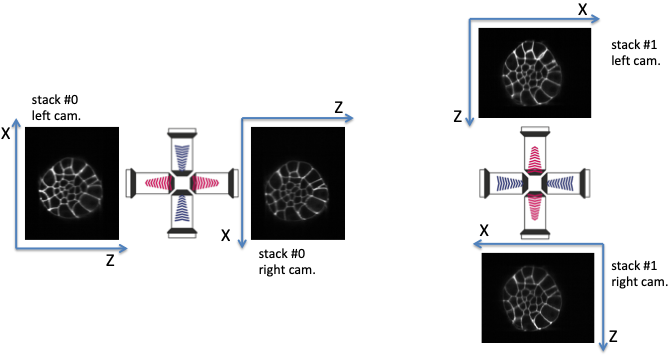
\includegraphics[width=150mm]{figures/acquisition-spim-right.png}
\end{center}
\caption{\label{fig:cli:fuse:spim:right:acquisition} Multiview lightsheet microscope acquisition: at a time point, two acquisitions (stack \#0 and stack \#1) are sequentially performed, the second one orthogonal to the first. For each acquisition, two 3D intensity image stacks are acquired, respectively by the left and the right cameras. 
It yields four image stacks to be fused. 
The frame $(\mathbf{X}, \mathbf{Z})$ of the left camera of stack \#0 needs to be rotated clockwise (90 degrees along the $\mathbf{Y}$ axis) to correspond to the frame of the left camera of stack \#1: \texttt{acquisition\_orientation} has to be set to \texttt{'right'} if \texttt{acquisition\_leftcamera\_z\_stacking} is set to \texttt{'direct'}.}
\end{figure}

\begin{figure}
\begin{center}
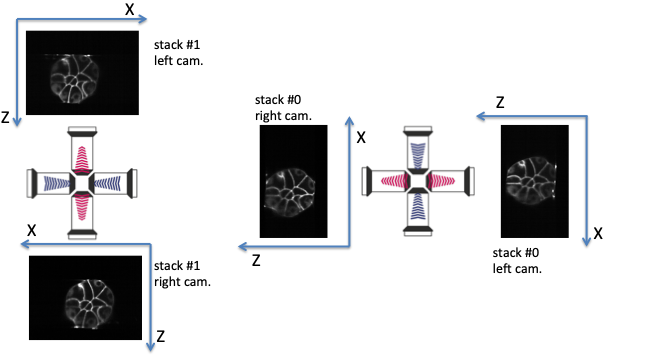
\includegraphics[width=150mm]{figures/acquisition-spim-left.png}
\end{center}
\caption{\label{fig:cli:fuse:spim:left:acquisition} The frame $(\mathbf{X}, \mathbf{Z})$ of the left camera of stack \#0 needs to be rotated counterclockwise (-90 degrees along the $\mathbf{Y}$ axis) to correspond to the frame of the left camera of stack \#1: \texttt{acquisition\_orientation} has to be set to \texttt{'left'} if \texttt{acquisition\_leftcamera\_z\_stacking} is set to \texttt{'direct'}.}
\end{figure}



\subsection{Important parameters in the parameter file}
\label{sec:cli:fuse:important:parameters}

A simple parameter file for fusion is described in the tutorial
section \ref{sec:tutorial:fusion}. A more comprehensive parameter file
example is provided in the \texttt{parameter-file-examples/} directory.

Indicating the right values of the
acquisition parameters is crucial; these parameters are
\begin{itemize}
\itemsep -0.5ex
\item \texttt{acquisition\_mirrors}  (or \texttt{raw\_mirrors}) is a parameter indicating whether the right camera images have already been mirrored along the X axis (so that the X axis direction is the one of the left cameras) or not. Its value is either \texttt{False} or \texttt{True}. Such a parameter should depend on the acquisition apparatus (ie the microscope) and the should be identical for all acquisitions.

In acquisitions depicted in figures \ref{fig:cli:fuse:spim:right:acquisition} and \ref{fig:cli:fuse:spim:left:acquisition}, it can be seen that the X-axis of the right camera image is inverted with respect to the left camera image. \texttt{acquisition\_mirrors} has to be set to \texttt{'False'}
  
  
\item \texttt{acquisition\_orientation} (or \texttt{raw\_ori}) is a parameter describing the acquisition orientation of the acquisition of the stack \#1 images with respect to the stack \#0 ones. 

\begin{itemize}
\itemsep -0.5ex
\item \texttt{'right'}: the frame $(\mathbf{X}, \mathbf{Z})$ of the left camera of stack \#0 needs to be rotated clockwise (90 degrees along the $\mathbf{Y}$ axis) to correspond to the left camera of stack \#1 (see figure \ref{fig:cli:fuse:spim:right:acquisition}).
\item \texttt{'left'}: the frame $(\mathbf{X}, \mathbf{Z})$ of the left camera of stack \#0 needs to be rotated counterclockwise (-90 degrees along the $\mathbf{Y}$ axis) to correspond to the left camera of stack \#1 (see figure \ref{fig:cli:fuse:spim:left:acquisition}).
\end{itemize}

\item \texttt{acquisition\_leftcamera\_z\_stacking}
 gives the order of stacking of in the Z direction for the left camera images.
\begin{itemize}
\itemsep -0.5ex
\item \texttt{'direct'}: \textbf{z} increases from the high-contrasted images to the blurred ones (see figure \ref{fig:cli:fuse:spim:right:acquisition}).
\item \texttt{'inverse'}: \textbf{z} increases from the blurred images to the high-contrasted ones (see figure \ref{fig:cli:fuse:spim:left:acquisition}).
\end{itemize}
Looking at XZ-sections of the registered images (see figures \ref{fig:cli:fuse:uniform:combination}, \ref{fig:cli:fuse:ramp:combination}, \ref{fig:cli:fuse:corner:combination}, and \ref{fig:cli:fuse:guignard:combination}) provides an efficient means to check whether this parameter is correctly set (see also section \ref{sec:cli:fuse:stack:fusion}).

\item \texttt{acquisition\_resolution} (or \texttt{raw\_resolution}) is the voxel size (along the 3
    dimensions X, Y and Z) of the acquired images.
\item \texttt{target\_resolution} is the desired isotropic (the
    same along the 3 dimensions) voxel size for the result fusion
    images.
\item \texttt{begin} gives the index of the first time point to be
  processed.
\item \texttt{end} gives the index of the last time point to be processed.
\end{itemize}


When one may not be sure of the \texttt{raw\_ori},
\texttt{raw\_mirrors}, and  \texttt{acquisition\_leftcamera\_z\_stacking}right values, it is advised to perform the
fusion on only one time point (by indicating the same index for both
\texttt{begin}  and \texttt{end}), e.g. with the four possibilities for the
variable couple (\texttt{raw\_ori}, \texttt{raw\_mirrors}), i.e.
(\texttt{'left'}, \texttt{False}),
(\texttt{'left'}, \texttt{True}),
(\texttt{'right'}, \texttt{False}), and
(\texttt{'right'}, \texttt{True}).
It comes to write four parameter files that differ only for the
parameters \texttt{raw\_ori}, \texttt{raw\_mirrors}, and
\texttt{EXP\_FUSE}  (to store the fusion result in different
directories, see section \ref{sec:cli:fuse:output:data}).
For these first experiments, it is advised 
\begin{itemize}
\itemsep -0.5ex
\item to set
\texttt{target\_resolution} to a large value, in order to speed up the
calculations, and
\item to set  \texttt{fusion\_xzsection\_extraction} to \texttt{True}, in order to check whether \texttt{acquisition\_leftcamera\_z\_stacking} was correctly set (see also section \ref{sec:cli:fuse:stack:fusion}).
\end{itemize}

Please recall that \texttt{raw\_ori} should depend on the acquisition apparatus (ie the microscope), and should not change for all the other acquisitions on the same microscope (unless the microscope settings change). Then, for most experiments, one change only to test the value of 
\texttt{raw\_ori}.

Please note that changing the value of \texttt{acquisition\_leftcamera\_z\_stacking} implies to change also the value of \texttt{acquisition\_orientation}.




\subsection{Input data}
\label{sec:cli:fuse:input:data}



Input data (acquired images from the MuViSPIM microscope, see figures \ref{fig:cli:fuse:spim:right:acquisition} and \ref{fig:cli:fuse:spim:left:acquisition}) are assumed
to be organized in a separate \texttt{RAWDATA/} directory in the 
\texttt{/path/to/experiment/} directory as depicted below. 
\begin{itemize}
  \itemsep -0.5ex
\item \texttt{RAWDATA/LC/Stack000} contains the images acquired at the
  first angulation by the left camera.
\item \texttt{RAWDATA/LC/Stack001} contains the images acquired at the
  second angulation by the left camera.
\item \texttt{RAWDATA/RC/Stack000} contains the images acquired at the
  first angulation by the right camera.
\item \texttt{RAWDATA/RC/Stack001} contains the images acquired at the
  second angulation by the right camera.
\end{itemize}

\mbox{}
\dirtree{%
.1 /path/to/experiment/.
.2 RAWDATA/.
.3 LC/.
.4 Stack0000/.
.5 Time000xxx\_00.zip.
.5 {\ldots}.
.5 Time000xxx\_00.zip.
.4 Stack0001/.
.5 Time000xxx\_00.zip.
.5 {\ldots}.
.5 Time000xxx\_00.zip.
.3 RC/.
.4 Stack0000/.
.5 Time000xxx\_00.zip.
.5 {\ldots}.
.5 Time000xxx\_00.zip.
.4 Stack0001/.
.5 Time000xxx\_00.zip.
.5 {\ldots}.
.5 Time000xxx\_00.zip.
.2 \ldots.
}
\mbox{}

where \texttt{xxx} denotes a three digit number (e.g. $000$, $001$,
...) denoting the time point of each acquisition. The range of time
points to be fused are given by the variables \texttt{begin} and
\texttt{end}, while the path \texttt{/path/to/experiment/} has to be
assigned to the variable \texttt{PATH\_EMBRYO} 

Hence a parameter file containing
\begin{verbatim}
PATH_EMBRYO = /path/to/experiment/
begin = 0
end = 10
\end{verbatim}
indicates that time points in $[0,10]$ of the \texttt{RAWDATA/}
subdirectory of  \texttt{/path/to/experiment/} have to be fused.

\subsubsection{Input data directory names}

However, directories may be named differently. The variables
\texttt{DIR\_RAWDATA}, \texttt{DIR\_LEFTCAM\_STACKZERO},
\texttt{DIR\_RIGHTCAM\_STACKZERO}, \texttt{DIR\_LEFTCAM\_STACKONE},
and \texttt{DIR\_RIGHTCAM\_STACKONE} allow a finer control of the
directory names. The images acquired at the first angulation by the
left and the right cameras are searched in the directories
\begin{verbatim}
<PATH_EMBRYO>/<DIR_RAWDATA>/<DIR_LEFTCAM_STACKZERO>
<PATH_EMBRYO>/<DIR_RAWDATA>/<DIR_RIGHTCAM_STACKZERO>
\end{verbatim}
while the images acquired at the second angulation by the
left and the right cameras are searched in the directories
\begin{verbatim}
<PATH_EMBRYO>/<DIR_RAWDATA>/<DIR_LEFTCAM_STACKONE>
<PATH_EMBRYO>/<DIR_RAWDATA>/<DIR_RIGHTCAM_STACKONE>
\end{verbatim}
where \texttt{<XXX>} denotes the value of the variable \texttt{XXX}.
Then, to parse the following data architecture

\mbox{}
\dirtree{%
.1 /path/to/experiment/.
.2 my\_raw\_data/.
.3 LeftCamera/.
.4 FirstStack/.
.5 {\ldots}.
.4 SecondStack/.
.5 {\ldots}.
.3 RightCamera/.
.4 FirstStack/.
.5 {\ldots}.
.4 SecondStack/.
.5 {\ldots}.
.2 \ldots.
}
\mbox{}

one has to add the following lines in the parameter file
\begin{verbatim}
DIR_RAWDATA = 'my_raw_data'
DIR_LEFTCAM_STACKZERO = 'LeftCamera/FirstStack'
DIR_RIGHTCAM_STACKZERO = 'RightCamera/FirstStack'
DIR_LEFTCAM_STACKONE = 'LeftCamera/SecondStack'
DIR_RIGHTCAM_STACKONE = 'RightCamera/SecondStack'
\end{verbatim}

It has to be noted that, when the stacks of a given time point are in
different directories, image file names are tried to be guessed from
the directories parsing. It has to be pointed out that indexes have to
be encoded with a 3-digit integer with 0 padding (i.e. $000$, $001$,
\ldots) and that has to be the only variation in the file names
(within each directory).

\subsubsection{Input data image file names}

Images acquired from the left and the right cameras may be stored in
the same directory, but obviously with different names as in 

\mbox{}
\dirtree{%
.1 /path/to/experiment/.
.2 RAWDATA/.
.3 stack\_0\_channel\_0.
.4 Cam\_Left\_00xxx.zip.
.4  \ldots .
.4 Cam\_Right\_00xxx.zip.
.4 \ldots .
.3 stack\_1\_channel\_0.
.4 Cam\_Left\_00xxx.zip.
.4  \ldots .
.4 Cam\_Right\_00xxx.zip.
.4 \ldots .
}
\mbox{}

The parameter file has then to contain the following lines to indicate
the directory names.
\begin{verbatim}
DIR_LEFTCAM_STACKZERO = 'stack_0_channel_0'
DIR_RIGHTCAM_STACKZERO = 'stack_0_channel_0'
DIR_LEFTCAM_STACKONE = 'stack_1_channel_0'
DIR_RIGHTCAM_STACKONE = 'stack_1_channel_0'
\end{verbatim}

In addition, to distinguish the images acquired by the left camera to
those acquired by the right one, one has to give the image name
prefixes, i.e. the common part of the image file names before the
3-digit number that indicates the time point.
This is the purpose of the  variables
\verb|acquisition_leftcam_image_prefix| and 
\verb|acquisition_rightcam_image_prefix|.
The parameter file has then to contain the following lines not only to indicate
the directory names but also the image file name prefixes.

\begin{verbatim}
DIR_LEFTCAM_STACKZERO = 'stack_0_channel_0'
DIR_RIGHTCAM_STACKZERO = 'stack_0_channel_0'
DIR_LEFTCAM_STACKONE = 'stack_1_channel_0'
DIR_RIGHTCAM_STACKONE = 'stack_1_channel_0'
acquisition_leftcam_image_prefix = 'Cam_Left_00'
acquisition_rightcam_image_prefix = 'Cam_Right_00'
\end{verbatim}

\subsubsection{Multichannel acquisition}

In case of multichannel acquisition, the fusion is computed for the
first channel, and the computed parameters (e.g. transformations,
etc.) are also used for the other channels. 

For a second channel, 
the images acquired at the first angulation by the
left and the right cameras are searched in the directories
\begin{verbatim}
<PATH_EMBRYO>/<DIR_RAWDATA>/<DIR_LEFTCAM_STACKZERO_CHANNEL_2>
<PATH_EMBRYO>/<DIR_RAWDATA>/<DIR_RIGHTCAM_STACKZERO_CHANNEL_2>
\end{verbatim}
while the images acquired at the second angulation by the
left and the right cameras are searched in the directories
\begin{verbatim}
<PATH_EMBRYO>/<DIR_RAWDATA>/<DIR_LEFTCAM_STACKONE_CHANNEL_2>
<PATH_EMBRYO>/<DIR_RAWDATA>/<DIR_RIGHTCAM_STACKONE_CHANNEL_2>
\end{verbatim}

For a third channel, 
the images acquired at the first angulation by the
left and the right cameras are searched in the directories
\begin{verbatim}
<PATH_EMBRYO>/<DIR_RAWDATA>/<DIR_LEFTCAM_STACKZERO_CHANNEL_3>
<PATH_EMBRYO>/<DIR_RAWDATA>/<DIR_RIGHTCAM_STACKZERO_CHANNEL_3>
\end{verbatim}
while the images acquired at the second angulation by the
left and the right cameras are searched in the directories
\begin{verbatim}
<PATH_EMBRYO>/<DIR_RAWDATA>/<DIR_LEFTCAM_STACKONE_CHANNEL_3>
<PATH_EMBRYO>/<DIR_RAWDATA>/<DIR_RIGHTCAM_STACKONE_CHANNEL_3>
\end{verbatim}



\subsection{Output data}
\label{sec:cli:fuse:output:data}

The variable \texttt{target\_resolution} allows to set the desired isotropic (the
same along the 3 dimensions) voxel size for the result fusion
images.

\subsubsection{Output data directory names}

The resulting fused images are stored in sub-directory
\texttt{FUSE/FUSE\_<EXP\_FUSE>} under the
\texttt{/path/to/experiment/} directory 

\mbox{}
\dirtree{%
.1 /path/to/experiment/.
.2 RAWDATA/.
.3 \ldots.
.2 FUSE/.
.3 FUSE\_<EXP\_FUSE>/.
.4 \ldots.
}
\mbox{}

where \texttt{<EXP\_FUSE>} is the value of the variable \texttt{EXP\_FUSE} (its
default value is '\texttt{RELEASE}'). Hence, the line
\begin{verbatim}
EXP_FUSE = 'TEST'
\end{verbatim}
in the parameter file will create the directory
\texttt{FUSE/FUSE\_TEST/} in which the fused images are stored. For
instance, when testing for the values of the variable couple
(\texttt{raw\_ori}, \texttt{raw\_mirrors}), a first parameter file may
contain
\begin{verbatim}
raw_ori = 'left'
raw_mirrors = False
begin = 1
end = 1
EXP_FUSE=TEST-LEFT-FALSE
\end{verbatim}
a second parameter file may
contain
\begin{verbatim}
raw_ori = 'left'
raw_mirrors = True
begin = 1
end = 1
EXP_FUSE=TEST-LEFT-TRUE
\end{verbatim}
etc. The resulting fused images will then be in different directories

\mbox{}
\dirtree{%
.1 /path/to/experiment/.
.2 RAWDATA/.
.3 \ldots.
.2 FUSE/.
.3 FUSE\_TEST-LEFT-FALSE/.
.4 \ldots.
.3 FUSE\_TEST-LEFT-TRUE/.
.4 \ldots.
.3 \ldots.
}
\mbox{}

This will ease their visual inspection to decide which values of the variable couple
(\texttt{raw\_ori}, \texttt{raw\_mirrors}) to use for the fusion.

\subsubsection{Output data file names}

Fused image files are named after the variable \texttt{EN}:
\texttt{<EN>\_fuse\_t<xxx>.inr} where \texttt{<xxx>} is the time point
index encoded by a 3-digit integer (with 0 padding).


\subsubsection{Multichannel acquisition}

Variables \texttt{EXP\_FUSE\_CHANNEL\_2} and
\texttt{EXP\_FUSE\_CHANNEL\_3} allows to set the directory names for
the resulting fused images of the other channels.

\subsection{Step \ref{it:fusion:crop:1} parameters: raw data cropping}
\label{sec:cli:fuse:raw:data:cropping}

For computational cost purposes, raw data (images acquired by the MuViSPIM microscope) are cropped (only in X and Y dimensions) before co-registration. A threshold is computed with Otsu's method \cite{otsu:tsmc:1979} on the maximum intensity projection (MIP) image. The cropping parameters are computed to keep the above-threshold points in the MIP image, plus some extra margins. Hyper-intense areas may biased the threshold computation, hence the cropping.

To desactivate this cropping, the line
\begin{verbatim}
raw_crop = False
\end{verbatim}
has to be added in the parameter file.

\subsection{Step \ref{it:fusion:registration} parameters: image co-registration}
\label{sec:cli:fuse:image:coregistration}

To fuse the images, they are co-registered onto a reference one. Co-registration are conducted only on the first channel (in case of multiple channel acquisitions), and the computed transformations are also applied onto the other channels. The reference image is chosen as being the acquisition from the left camera for the first stack (also denoted stack \#0). The co-registration strategy is given by the variable \texttt{fusion\_strategy} in the parameter file.


\subsubsection{Fusion \textit{direct} strategy}

\begin{figure}
\begin{center}
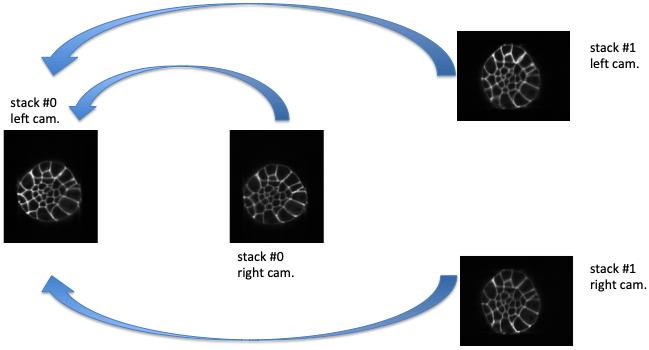
\includegraphics[height=50mm]{figures/fusion-direct-strategy.png}
\end{center}
\caption{\label{fig:cli:fuse:direct:strategy} Fusion \textit{direct} strategy: each 3D image is co-registered on the reference one, chosen here as the left camera image of stack \#0.}
\end{figure}

In the parameter file, the line
\begin{verbatim}
fusion_strategy = 'direct-fusion'
\end{verbatim}
will set the co-registration strategy to the one described in \cite{guignard:tel-01278725,guignard:hal-01938126}: each acquisition image is linearly co-registered with the reference one, i.e. the one from the left camera and for the first stack.

Let us denote by $I^{0}_{LC}$ the left camera image of stack\#0, the three other images are $I^{0}_{RC}$, $I^{1}_{LC}$, and $I^{1}_{RC}$. By (linear) co-registration (see section \ref{sec:cli:fuse:acquisition:registration}) of these image with $I^{0}_{LC}$, the 3 transformations
$T_{I^{0}_{RC} \leftarrow I^{0}_{LC}}$,
$T_{I^{1}_{LC} \leftarrow I^{0}_{LC}}$, and
$T_{I^{1}_{RC} \leftarrow I^{0}_{LC}}$
are computed.
$T_{I^{0}_{RC} \leftarrow I^{0}_{LC}}$ is the transformation that allows to resample $I^{0}_{RC}$ in the same frame than $I^{0}_{LC}$:
$I^{0}_{RC} \circ T_{I^{0}_{RC} \leftarrow I^{0}_{LC}}$ denotes this resampled image.


\subsubsection{Fusion \textit{hierarchical} strategy}

\begin{figure}
\begin{center}
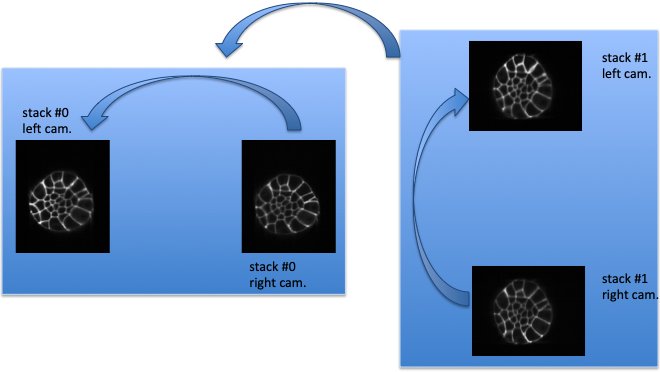
\includegraphics[height=50mm]{figures/fusion-hierarchical-strategy.png}  
\end{center}
\caption{\label{fig:cli:fuse:hierarchical:strategy} Fusion \textit{hierarchical} strategy. Stacks \#0 and \#1 are reconstructed independently: right camera images are co-registered on the left camera ones, and stacks \#0 and \#1 are reconstructed by fusing left and right camera images. Fused image of stack \#1 is co-registered on fused image of stack \#0: by transformation composition, it allows to compute the transformations of left and right camera images of stack \#1 onto the left camera image of stack \#0.}
\end{figure}

In the parameter file, the line
\begin{verbatim}
fusion_strategy = 'hierarchical-fusion'
\end{verbatim}
defines a hierarchical  co-registration  strategy. First, the right camera image of each stack is linearly co-registered (see section \ref{sec:cli:fuse:acquisition:registration}) on its left camera counterpart, yielding the transformations
$T_{I^{0}_{RC} \leftarrow I^{0}_{LC}}$ and
$T_{I^{1}_{RC} \leftarrow I^{1}_{LC}}$.
According that the left and right camera images of a stack are acquired simultaneously, a linear transformation is then completely adequate to co-register them.

This allows to fuse (see section \ref{sec:cli:fuse:stack:fusion}) the two acquisition of the corresponding left and right cameras into a single stack:
\begin{eqnarray*}
I^{0} & = & \omega^{0}_{LC} I^{0}_{LC} 
          + \omega^{0}_{RC} I^{0}_{RC} \circ T_{I^{0}_{RC} \leftarrow I^{0}_{LC}} \quad \textrm{and} \\
I^{1} & = & \omega^{1}_{LC} I^{1}_{LC} 
          + \omega^{1}_{RC} I^{1}_{RC} \circ T_{I^{1}_{RC} \leftarrow I^{1}_{LC}}                         
\end{eqnarray*}

The reconstructed stacks are then (potentially non-linearly, see section \ref{sec:cli:fuse:stack:registration}) co-registered together, yielding the transformation $T_{I^{1} \leftarrow I^{0}}$. This allows to get the 
$T_{I^{1}_{RC} \leftarrow I^{0}_{RC}}$ and
$T_{I^{1}_{LC} \leftarrow I^{0}_{RC}}$ transformations 
\begin{eqnarray*}
T_{I^{1}_{LC} \leftarrow I^{0}_{LC}} & = & T_{I^{1} \leftarrow I^{0}} \quad \textrm{and} \\
T_{I^{1}_{RC} \leftarrow I^{0}_{LC}} & = &
T_{I^{1}_{RC} \leftarrow I^{1}_{LC}} \circ T_{I^{1} \leftarrow I^{0}}                      
\end{eqnarray*}
Using a non-linear registration in this last step allows to compensate for some distortions that may occur between the two stacks \#0 and \#1. Please note that stack \#0 is then assumed to be the non-distorted reference while left and right camera image of stack \#1 will be deformed before fusion.


\subsubsection{Acquisitions linear co-registration}
\label{sec:cli:fuse:acquisition:registration}
The linear co-registrations are either used to co-registered each acquisition onto the reference one in the \texttt{'direct-fusion'} strategy, or to build stacks from the left and right cameras in the \texttt{'hierarchical-fusion'} strategy.
Variables that controls the linear co-registrations are either prefixed by \texttt{fusion\_preregistration\_} or by \texttt{fusion\_registration\_}.

To decrease the computational cost, images are normalized and cast on one byte before registration. While it generally does not degrade the registration quality, it may induce troubles when hyper-intensities areas are present in the image. In such a case, the useful information may then be summarized in only a few intensity values.

Intensity normalization in registration can be deactivated by adding the following line in the parameter file
\begin{verbatim}
fusion_registration_normalization = False
\end{verbatim}

To verify whether a good quality registration can be conducted, the searched transformation type can be changed for a simpler one than affine. 
Adding the following line in the parameter file.
\begin{verbatim}
fusion_registration_transformation_type = translation
\end{verbatim}
will search for a translation which could be supposed to be sufficient, according that only translations relates the 4 acquisitions of the MuViSPIM microscope (in a perfect setting). If the search for an affine transformation (the default behavior) failed (the fusion looks poor) while the search for a translation is successful (the fusion looks good), a two-steps registration may help to refine the found translation by a subsequent affine transformation as explained below.

Hyper-intensities areas may also bias the threshold calculation used for the automatic crop (step \ref{it:fusion:crop:1} of fusion). In such cases, the iterative registration method may find a local minimum that is not the desired one, because the relative positions of the two images to be co-registered are too far apart. To circumvent such a behavior, a two-steps registration can be done. It consists on a first pre-registration with a transformation with fewer degrees of freedom (i.e. a 3D translation). 

This pre-registration can be activated by adding the following line in the parameter file.
\begin{verbatim}
fusion_preregistration_compute_registration = True
\end{verbatim}
It may be also preferable to deactivate the image normalization for both registration steps with
\begin{verbatim}
fusion_preregistration_normalization = False
fusion_registration_normalization = False
\end{verbatim}

\subsubsection{Stacks non-linear co-registration}
\label{sec:cli:fuse:stack:registration}
Variables that controls the non-linear co-registrations are either prefixed by \texttt{fusion\_stack\_preregistration\_} or by \texttt{fusion\_stack\_registration\_}. They are defined similarly as the one of acquisitions co-registration. 






\subsection{Step \ref{it:fusion:combination}: linear combination of co-registered image stacks}
\label{sec:cli:fuse:stack:fusion}

The resampled co-registered image stacks are fused together by the means of a weighted linear combination.
\begin{displaymath}
I_{fuse} =
\omega^{0}_{LC} I^{0}_{LC}
+ \omega^{0}_{RC} I^{0}_{RC} \circ T_{I^{0}_{RC} \leftarrow I^{0}_{LC}}
+ \omega^{1}_{LC} I^{1}_{LC} \circ T_{I^{1}_{LC} \leftarrow I^{0}_{LC}}
+ \omega^{1}_{RC} I^{1}_{RC} \circ T_{I^{1}_{RC} \leftarrow I^{0}_{LC}}
\end{displaymath}



\begin{figure}
\begin{center}
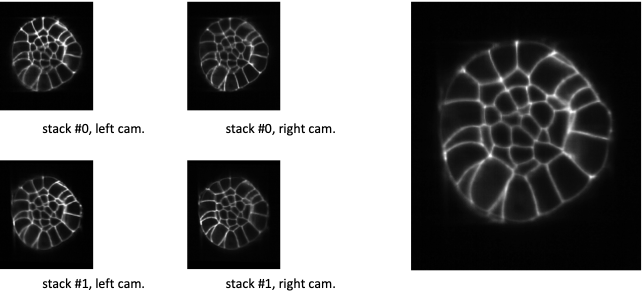
\includegraphics[height=50mm]{figures/fusion-uniform-combination.png}
\end{center}
\caption{\label{fig:cli:fuse:uniform:combination} At the left, XZ-sections of 4 co-registered stacks. 
At the right, the linear combination of the 4 co-registered stacks with an uniform (or constant) weighting function. It comes to make an average of the 4 co-registered stacks.}
\end{figure}

\begin{figure}
\begin{center}
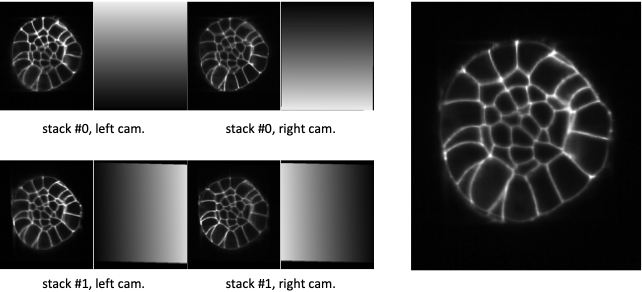
\includegraphics[height=50mm]{figures/fusion-ramp-combination.png}
\end{center}
\caption{\label{fig:cli:fuse:ramp:combination} At the left, XZ-sections of 4 co-registered stacks together with their ramp weighting function.
At the right, the linear combination of the 4 co-registered stacks with this ramp weighting function.}
\end{figure}

\begin{figure}
\begin{center}
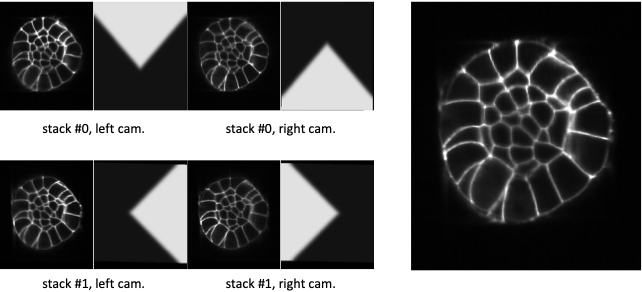
\includegraphics[height=50mm]{figures/fusion-corner-combination.png}
\end{center}
\caption{\label{fig:cli:fuse:corner:combination} At the left, XZ-sections of 4 co-registered stacks together with their corner weighting function.
At the right, the linear combination of the 4 co-registered stacks with this corner weighting function.}
\end{figure}

\begin{figure}
\begin{center}
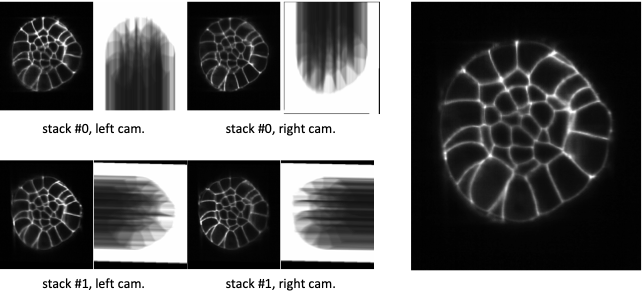
\includegraphics[height=50mm]{figures/fusion-guignard-combination.png}
\end{center}
\caption{\label{fig:cli:fuse:guignard:combination} At the left, XZ-sections of 4 co-registered stacks together with their Guignard's weighting function.
At the right, the linear combination of the 4 co-registered stacks with this weighting function.}
\end{figure}



The choice of the weighting function is controlled by the variable \texttt{fusion\_weighting}, eventually suffixed by \texttt{\_channel\_[1,2,3]} if one wants to use different weighting schemes for the different channels to be fused.


The variable \texttt{fusion\_weighting} can be set to

\begin{itemize}
\item \texttt{'uniform'}:
it comes to the average of the resampled co-registered stacks (see figure \ref{fig:cli:fuse:uniform:combination}). Such a weighting does not depend on the stacks to be fused.
\item \texttt{'ramp'}:
the weights are linearly increasing along the \textbf{Z} axis (see figure \ref{fig:cli:fuse:ramp:combination}).
\item \texttt{'corner'}: the weights are constant in a corner portion of the stack, defined by two diagonals in the \textbf{XZ}-section (see figure \ref{fig:cli:fuse:corner:combination}). It somehow mimics a stitching of the 4 resampled co-registered image stacks, where the information is kept from the most informative image.
\item \texttt{'guignard'}: 
the weighting function is the one described in \cite{guignard:tel-01278725}.
More weight are given to sections close to the camera and it also takes into account the traversed material (see figure \ref{fig:cli:fuse:guignard:combination}). 
\end{itemize} 

Weighting functions are designed so that the weights decrease with \textbf{Z} for the left camera images and increase with \textbf{Z} for the left camera images. So, setting the \texttt{acquisition\_leftcamera\_z\_stacking} variable to the wrong value (\texttt{'direct'} instead of \texttt{'inverse'}, or vice-versa) may then decrease the fusion quality. 

Looking at XZ-sections of the co-registered image stacks, as well as the weighting function images, (see figures \ref{fig:cli:fuse:uniform:combination}, \ref{fig:cli:fuse:ramp:combination}, \ref{fig:cli:fuse:corner:combination}, and \ref{fig:cli:fuse:guignard:combination}) provides a direct and efficient means to check whether this parameter is correctly set. Such sections can be extracted by setting the \texttt{fusion\_xzsection\_extraction} parameter to \texttt{True}. It creates \texttt{XZSECTION\_<xxx>/} subdirectories (one par time point, \texttt{<xxx>} being the time point index) in the \texttt{FUSE/FUSE\_<EXP\_FUSE>/} directory.

\mbox{}
\dirtree{%
.1 /path/to/experiment/.
.2 RAWDATA/.
.3 \ldots.
.2 FUSE/.
.3 FUSE\_<EXP\_FUSE>/.
.4 \ldots.
.4 XZSECTION\_<xxx>/.
.4 \ldots.
}
\mbox{}


When using the variable \texttt{fusion\_weighting}, the same weights (computed on the first channel to be processed) are used for all fusion. However, different weighting functions can be used for the channels to be fused by using the variables  \texttt{fusion\_weighting\_channel\_[1,2,3]}, eg
\begin{verbatim}
fusion_weighting_channel_1 = 'guignard'
fusion_weighting_channel_2 = 'uniform'
\end{verbatim}


\subsection{Step \ref{it:fusion:crop:2}: fused data cropping}
\label{sec:cli:fuse:fused:data:cropping}

To save disk storage, fused images are cropped at the end of the fusion stage. To desactivate this cropping, the line
\begin{verbatim}
fusion_crop = False
\end{verbatim}
has to be added in the parameter file.

\subsection{Troubleshooting}

\begin{itemize}

\item The fused images are obviously wrong.
  \begin{enumerate}
  \item Are the values of the variable couple (\texttt{raw\_ori}, \texttt{raw\_mirrors}) the right ones? Conduct experiments as suggested in section \ref{sec:cli:fuse:important:parameters}  (see also section \ref{sec:cli:fuse:output:data}) to get the right values.
  \item The registration may have failed.
    \begin{enumerate}
    \item Deactivate the 1-byte normalization (see section \ref{sec:cli:fuse:image:coregistration}).
    \item Try to register with a simpler transformation type (i.e. translation) and/or with a two-steps registration (see section \ref{sec:cli:fuse:image:coregistration}).
    \end{enumerate}
  \end{enumerate}
\item The imaged sample is cropped by the image border in the fused image.
  \begin{enumerate}
  \item Check whether the imaged sample was not already cropped in the raw data.
  \item The automated cropping may have failed. It is more likely to happen when cropping the raw data, so deactivate it (see section \ref{sec:cli:fuse:raw:data:cropping}). If it still happens, try to deactivate also the fused image cropping   (see section \ref{sec:cli:fuse:fused:data:cropping}).
  \end{enumerate}
\end{itemize}

\subsection{Parameter list}

Please also refer to the file
\texttt{parameter-file-examples/1-fuse-parameters.py}

\begin{itemize}
\itemsep -0.5ex
\item \texttt{DIR\_LEFTCAM\_STACKONE} see section \ref{sec:cli:fuse:input:data}
\item \texttt{DIR\_LEFTCAM\_STACKONE\_CHANNEL\_2} see section \ref{sec:cli:fuse:input:data}
\item \texttt{DIR\_LEFTCAM\_STACKONE\_CHANNEL\_3} see section \ref{sec:cli:fuse:input:data}
\item \texttt{DIR\_LEFTCAM\_STACKZERO} see section \ref{sec:cli:fuse:input:data}
\item \texttt{DIR\_LEFTCAM\_STACKZERO\_CHANNEL\_2} see section \ref{sec:cli:fuse:input:data}
\item \texttt{DIR\_LEFTCAM\_STACKZERO\_CHANNEL\_3} see section \ref{sec:cli:fuse:input:data}
\item \texttt{DIR\_RAWDATA} see section \ref{sec:cli:fuse:input:data}
\item \texttt{DIR\_RAWDATA\_CHANNEL\_2} see section \ref{sec:cli:fuse:input:data}
\item \texttt{DIR\_RAWDATA\_CHANNEL\_3} see section \ref{sec:cli:fuse:input:data}
\item \texttt{DIR\_RIGHTCAM\_STACKONE} see section \ref{sec:cli:fuse:input:data}
\item \texttt{DIR\_RIGHTCAM\_STACKONE\_CHANNEL\_2} see section \ref{sec:cli:fuse:input:data}
\item \texttt{DIR\_RIGHTCAM\_STACKONE\_CHANNEL\_3} see section \ref{sec:cli:fuse:input:data}
\item \texttt{DIR\_RIGHTCAM\_STACKZERO} see section \ref{sec:cli:fuse:input:data}
\item \texttt{DIR\_RIGHTCAM\_STACKZERO\_CHANNEL\_2} see section \ref{sec:cli:fuse:input:data}
\item \texttt{DIR\_RIGHTCAM\_STACKZERO\_CHANNEL\_3} see section \ref{sec:cli:fuse:input:data}
\item \texttt{EN} see section \ref{sec:cli:fuse:output:data}
\item \texttt{EXP\_FUSE} see section \ref{sec:cli:fuse:output:data}
\item \texttt{EXP\_FUSE\_CHANNEL\_2} see section \ref{sec:cli:fuse:output:data}
\item \texttt{EXP\_FUSE\_CHANNEL\_3} see section \ref{sec:cli:fuse:output:data}
\item \texttt{PATH\_EMBRYO} see section \ref{sec:cli:fuse:input:data}
\item \texttt{RESULT\_IMAGE\_SUFFIX\_FUSE}
\item \texttt{acquisition\_leftcam\_image\_prefix}  see section \ref{sec:cli:fuse:input:data}
\item \texttt{acquisition\_leftcamera\_z\_stacking}
\item \texttt{acquisition\_mirrors} same as \texttt{raw\_mirrors}
\item \texttt{acquisition\_orientation} same as \texttt{raw\_ori}
\item \texttt{acquisition\_resolution} same as \texttt{raw\_resolution}
\item \texttt{acquisition\_rightcam\_image\_prefix}  see section \ref{sec:cli:fuse:input:data}
\item \texttt{acquisition\_slit\_line\_correction}
\item \texttt{begin} see section \ref{sec:cli:fuse:important:parameters}
\item \texttt{default\_image\_suffix}
\item \texttt{delta}
\item \texttt{end} see section \ref{sec:cli:fuse:important:parameters}
\item \texttt{fusion\_crop} see section \ref{sec:cli:fuse:fused:data:cropping}
\item \texttt{fusion\_margin\_x\_0}
\item \texttt{fusion\_margin\_x\_1}
\item \texttt{fusion\_margin\_y\_0}
\item \texttt{fusion\_margin\_y\_1}
\item \texttt{fusion\_strategy}  see section \ref{sec:cli:fuse:image:coregistration}
\item \texttt{fusion\_preregistration\_compute\_registration} see section \ref{sec:cli:fuse:image:coregistration}
\item \texttt{fusion\_preregistration\_lts\_fraction}
\item \texttt{fusion\_preregistration\_normalization} see section \ref{sec:cli:fuse:image:coregistration}
\item \texttt{fusion\_preregistration\_pyramid\_highest\_level}
\item \texttt{fusion\_preregistration\_pyramid\_lowest\_level}
\item \texttt{fusion\_preregistration\_transformation\_estimation\_type}
\item \texttt{fusion\_preregistration\_transformation\_type}
\item \texttt{fusion\_registration\_compute\_registration}
\item \texttt{fusion\_registration\_lts\_fraction}
\item \texttt{fusion\_registration\_normalization} see section \ref{sec:cli:fuse:image:coregistration}
\item \texttt{fusion\_registration\_pyramid\_highest\_level}
\item \texttt{fusion\_registration\_pyramid\_lowest\_level}
\item \texttt{fusion\_registration\_transformation\_estimation\_type}
\item \texttt{fusion\_registration\_transformation\_type} see section \ref{sec:cli:fuse:image:coregistration}
\item \texttt{fusion\_stack\_preregistration\_compute\_registration}
\item \texttt{fusion\_stack\_preregistration\_lts\_fraction}
\item \texttt{fusion\_stack\_preregistration\_normalization}
\item \texttt{fusion\_stack\_preregistration\_pyramid\_highest\_level}
\item \texttt{fusion\_stack\_preregistration\_pyramid\_lowest\_level}
\item \texttt{fusion\_stack\_preregistration\_transformation\_estimation\_type}
\item \texttt{fusion\_stack\_preregistration\_transformation\_type}
\item \texttt{fusion\_stack\_registration\_compute\_registration}
\item \texttt{fusion\_stack\_registration\_lts\_fraction}
\item \texttt{fusion\_stack\_registration\_normalization}
\item \texttt{fusion\_stack\_registration\_pyramid\_highest\_level}
\item \texttt{fusion\_stack\_registration\_pyramid\_lowest\_level}
\item \texttt{fusion\_stack\_registration\_transformation\_estimation\_type}
\item \texttt{fusion\_stack\_registration\_transformation\_type}
\item \texttt{fusion\_weighting}
\item \texttt{fusion\_weighting\_channel\_1}
\item \texttt{fusion\_weighting\_channel\_2}
\item \texttt{fusion\_weighting\_channel\_3}
\item \texttt{fusion\_xzsection\_extraction} see section \ref{sec:cli:fuse:stack:fusion}
\item \texttt{raw\_crop} see section \ref{sec:cli:fuse:raw:data:cropping}
\item \texttt{raw\_delay}
\item \texttt{raw\_leftcamera\_z\_stacking}
\item \texttt{raw\_margin\_x\_0}
\item \texttt{raw\_margin\_x\_1}
\item \texttt{raw\_margin\_y\_0}
\item \texttt{raw\_margin\_y\_1}
\item \texttt{raw\_mirrors} see section \ref{sec:cli:fuse:important:parameters}
\item \texttt{raw\_ori} see section \ref{sec:cli:fuse:important:parameters}
\item \texttt{raw\_resolution} see section \ref{sec:cli:fuse:important:parameters}
\item \texttt{result\_image\_suffix}
\item \texttt{target\_resolution} see section \ref{sec:cli:fuse:output:data}
\end{itemize}


%%%%%%%%%%%%%%%%%%%%%%%%%%%%%%%%%%%%%%%%%%%%%%%%%%%%%%%%%%%%
%
% 1.5-intraregistration.py
%
%%%%%%%%%%%%%%%%%%%%%%%%%%%%%%%%%%%%%%%%%%%%%%%%%%%%%%%%%%%%

\section{\texttt{1.5-intraregistration.py}}
\label{sec:cli:intraregistration}

The sequence intra-registration procedure can be done either after the fusion step, or after the (post-)segmentation step. It aims at
\begin{itemize}
\itemsep -1ex
\item compensating for the eventual motion of the imaged sample with respect to the microscope
\item resampling the fusion and/or the segmentation images into a common frame/geometry, so they can better be compared, and
\item building 2D+t images made of 2D sections from either the  fusion
  and/or the segmentation images, so that the quality of the fusion
  and/of the tracking step can be visually assessed. 
\end{itemize}


The intra-registration procedure is made of the following steps:
\begin{enumerate}
\itemsep -1ex
\item \label{it:intrareg:co:register} Co-registration of pairs of successive fused images (section
  \ref{sec:cli:intraregistration:coregistration}). This yields the
  transformations $T_{t+1 \leftarrow t}$. Fused images are located in
  \verb|<EMBRYO>/FUSE/FUSE_<EXP_FUSE>|: the parameter \verb|EXP_FUSE|
  is either set in the parameter file or is set at
  \verb|RELEASE|. This step may be long. 

\item Composition of transformations issued from the co-registration
  step. This step computes the transformations $T_{ref \leftarrow
    t}$. towards a reference image \verb|ref| given by the parameter
  \verb|intra_registration_reference_index|. 

\item \label{it:intrareg:co:template} Computation of the \textit{template} image (section
  \ref{sec:cli:intraregistration:template}). This \textit{template}
  image dimension are computed so that the useful information of all
  resampled images fits into it. Useful information can be issued from
  either the fused sequence, the segmentation sequence or the
  post-segmentation sequence. It is indicated by the
  \verb|intra_registration_template_type| which value can be either
  \verb|'FUSION'|,  \verb|'SEGMENTATION'|, or
  \verb|'POST-SEGMENTATION'|. This step may be long. 

\item \label{it:intrareg:co:resampling}
  Resampling of either the fused or the segmentation images
  (section \ref{sec:cli:intraregistration:resampling}). Note that
  changing the parameters for this step will not require to re-compute
  the first steps. 

\item \label{it:intrareg:co:movies}
  Extraction of 2D+t images from the resampled sequences (section
  \ref{sec:cli:intraregistration:movies}). Note that changing the
  parameters for this step (i.e. requiring extra movies) will not
  require to re-compute the first steps, with an eventual exception
  for the resampling step. 

\item \label{it:intrareg:co:maximum}
  Computation of a maximum image from the resampled images (section
  \ref{sec:cli:intraregistration:maximum}). Computing the maximum over  
  the resampled fusion images may be useful to define a common cropping
  area for the sequence.
  Note that changing the parameters for this step will not require 
  to re-compute the first steps. 

\end{enumerate}



\subsection{\texttt{1.5-intraregistration.py} options}

The following options are available:
\begin{description}
  \itemsep -1ex
\item[\texttt{-h}] prints a help message
\item[\texttt{-p \underline{file}}] set the parameter file to be parsed
\item[\texttt{-e \underline{path}}] set the
  \texttt{\underline{path}} to the directory where the
  \texttt{RAWDATA/} directory is located
\item[\texttt{-t \underline{file}}] set the resampling transformation file for the reference image (see section \ref{sec:cli:intraregistration:template})
\item[\texttt{-a \underline{string}}] set the resampling transformation angles for the reference image (see section \ref{sec:cli:intraregistration:template})
\item[\texttt{-k}] allows to keep the temporary files
\item[\texttt{-f}] forces execution, even if (temporary) result files
  are already existing
\item[\texttt{-v}] increases verboseness (both at console and in the
  log file)
\item[\texttt{-nv}] no verboseness
\item[\texttt{-d}]  increases debug information (in the
  log file)
\item[\texttt{-nd}] no debug information
\end{description}


\subsection{Output data}

The results are stored in sub-directories
\texttt{INTRAREG/INTRAREG\_<EXP\_INTRAREG>} under the
\texttt{/path/to/experiment/} directory where \texttt{<EXP\_INTRAREG>} is the value of the variable \texttt{EXP\_INTRAREG} (its
default value is '\texttt{RELEASE}'). 

\mbox{}
\dirtree{%
.1 /path/to/experiment/.
.2 \ldots.
.2 INTRAREG/.
.3 INTRAREG\_<EXP\_INTRAREG>/.
.4 CO-TRSFS/.
.4 [FUSE/].
.4 LOGS/.
.4 [MAXIMUM/].
.4 [MOVIES/].
.4 [POST/].
.4 [SEG/].
.4 TRSFS\_t<begin>-<end>/.
.2 \ldots.
}
\mbox{}

Output data are of two kinds: image series (fused images, segmentation
images, post-corrected segmentation images) can be resampled in the
same common geometry (also known as the \textit{template}), see
section \ref{sec:cli:intraregistration:resampling}, and 3D (ie 2D+t)
images of the evolution (with respect to time) of one section (XY, XZ,
or YZ) of the images of the series can be built, see
section \ref{sec:cli:intraregistration:movies}.




\subsection{Intra-registration parameters}

\subsubsection{Step \ref{it:intrareg:co:register}: co-registration}
\label{sec:cli:intraregistration:coregistration}
Default registration parameters for the co-registration are set by:
\begin{verbatim}
# intra_registration_compute_registration = True
# intra_registration_transformation_type = 'rigid'
# intra_registration_transformation_estimation_type = 'wlts'
# intra_registration_lts_fraction = 0.55
# intra_registration_pyramid_highest_level = 6
# intra_registration_pyramid_lowest_level = 3
# intra_registration_normalization = True
\end{verbatim}
Computed transformations are stored in \verb|INTRAREG/INTRAREG_<EXP\_INTRAREG>/CO-TRSFS|.
It may be advised to set the pyramid lowest level value to some higher value to speed up the co-registrations (recall that all pairs of successive images will be co-registered, i.e.
\begin{verbatim}
intra_registration_pyramid_lowest_level = 4
\end{verbatim}

Co-registration are computed using the fused images of
\texttt{/path/to/experiment/FUSE/FUSE\_<EXP\_FUSE>}. If
\texttt{EXP\_FUSE} is a list of strings (ie indicates a list a
directories) rather than a single string, the fused image from the
first directory are used for the co-registration computation.

Typically, if there are several fused series (eg, in case of multi-channel
acquisition) as in

\mbox{}
\dirtree{%
.1 /path/to/experiment/.
.2 \ldots.
.2 FUSE/.
.3 FUSE\_MEMBRANES/.
.3 FUSE\_NUCLEI/.
.2 \ldots.
}
\mbox{}

Specifying
\begin{verbatim}
EXP_FUSE = ['MEMBRANES', 'NUCLEI']
\end{verbatim}
in the parameter file implies that co-registrations will be done on
the fused images from \texttt{FUSE/FUSE\_MEMBRANES/}.



\subsubsection{Step \ref{it:intrareg:co:template}: template building}
\label{sec:cli:intraregistration:template}

\begin{verbatim}
# intra_registration_reference_index = None
# intra_registration_reference_resampling_transformation_file = None
# intra_registration_reference_resampling_transformation_angles = None
#
# intra_registration_template_type = "FUSION"
# intra_registration_template_threshold = None
# intra_registration_margin = None
#
# intra_registration_resolution = 0.6
#
# intra_registration_rebuild_template = False
\end{verbatim}

\begin{itemize}
\itemsep -1ex

\item The \verb|intra_registration_reference_index| allows to choose the reference image (the one which remains still, i.e. up to a translation), by default it is the first image image of the series (associated to \verb|begin|). 
However, it may happen that this image has to be reoriented to fit the user's expectation. The resampling transformation\footnote{The resampling transformation is the one that goes from the destination image towards the input image.}, that re-orient the reference image, can then be given and will be applied to the whole series.
\begin{itemize}
\itemsep -1ex
\item \verb|intra_registration_reference_resampling_transformation_file| can be given a resampling transformation file name.
\item \verb|intra_registration_reference_resampling_transformation_angles| can be given a string describing the successive rotations (with respect to the frame axis) to be applied. E.g. the string \verb|"X 30 Y 50"| defines a resampling transformation equal to $R_X(30) \circ R_Y(50)$ where $R_X(30)$ is a rotation of 30 degrees around the X axis and $R_Y(50)$ is a rotation of 50 degrees around the Y axis.
\end{itemize}

\item Depending on \verb|intra_registration_template_type| (\verb|'FUSION'|,
\verb|'SEGMENTATION'| or \verb|'POST-SEGMENTATION'|), the two latter
assume obviously that the segmentation has been done), the
\textit{template} image can be built either after the fusion or the
segmentation images. If no threshold is given by
\verb|intra_registration_template_threshold|, the built template will
be large enough to include all the transformed fields of view (in this
case, the template is the same whatever
\verb|intra_registration_template_type| is).

If \verb|intra_registration_template_type='FUSION'| (respectively
\verb|'SEGMENTATION'| and \verb|'POST-SEGMENTATION'|),  the template
is built from the images of the first directory indicated by
\texttt{EXP\_FUSE} (respectively
\texttt{EXP\_SEG} and \texttt{EXP\_POST}) in case of
\texttt{EXP\_FUSE} contains a list of strings.

If a threshold is given, the built template will be large enough to
include all the transformed points above the threshold. E.g., the
background is labeled with either '1' or '0' in segmentation images,
then a threshold of '2' ensures that all the embryo cells will not be
cut by the resampling stage.  In this case, adding an additional
margin (with \verb|intra_registration_margin|) to the template could be a good idea for visualization
purpose. 

\item Specifying  using a different resolution for the drift-compensated series than the
\verb|target_resolution| (the resolution of the fused images) allows
to decrease the resampled images volume. This can be achieved by
setting \verb|intra_registration_resolution| to the desired  value  (default is 0.6).

\item 
Last, co-registrations may have been computed during a first
computation, fused images being used to compute the template. However,
if  a subsequent segmentation has been conducted, a smaller template
is likely to be computed (with the segmentation images to build the
template), without recomputing the co-registration. This is the
purpose of the variable
\texttt{intra\_registration\_rebuild\_template}.
If set to \texttt{True}, it forces to recompute the template as well
as the transformations from the co-registrations (that are not
re-computed). Obviously, resampling as well as 2D+t movies are also
re-generated.
\end{itemize}

As an example, building a \textit{template} image after the segmentation images can be done with
\begin{verbatim}
# intra_registration_reference_index = None
intra_registration_template_type = "SEGMENTATION"
intra_registration_template_threshold = 2
# intra_registration_resolution = 0.6
intra_registration_margin = 10
\end{verbatim}


Computed transformations from the \textit{template} image as well as the \textit{template} image itself are stored in \verb|INTRAREG/INTRAREG<EXP_INTRAREG>/TRSFS_t<F>-<L>/| where \verb|<F>| and \verb|L| are the first and the last index of the series (specified by \verb|begin| and \verb|end| from the parameter file).


\subsubsection{Step \ref{it:intrareg:co:resampling}: resampling fusion/segmentation images}
\label{sec:cli:intraregistration:resampling}

The resampling of the fused and/or segmentation images are done
depending on the value of the following variables (here commented). Resampling is done
either if the following parameters are set to \verb|True| or if movies
are requested to be computed (section \ref{sec:cli:intraregistration:movies}).
\begin{verbatim}
# intra_registration_resample_fusion_images = True
# intra_registration_resample_segmentation_images = False
# intra_registration_resample_post_segmentation_images = False
\end{verbatim}
This default behavior implies that the fusion images will be resampled
while the segmentation and the post-corrected segmentation images are not.


Resampled images will be stored in the
\texttt{INTRAREG/INTRAREG\_<EXP\_INTRAREG/>} directory, with the same
hierarchy than under \texttt{/path/to/experiment}. E.g. 

\mbox{}
\dirtree{%
.1 /path/to/experiment/.
.2 \ldots.
.2 FUSE/.
.3 FUSE\_1/.
.3 FUSE\_2/.
.2 \ldots.
}
\mbox{}

Specifying
\begin{verbatim}
EXP_FUSE = ['1', '2']
\end{verbatim}
in the parameter file causes the resampling of both fused image series
(\texttt{FUSE/FUSE\_1/} and \texttt{FUSE/FUSE\_2/})

\mbox{}
\dirtree{%
.1 /path/to/experiment/.
.2 \ldots.
.2 FUSE/.
.3 FUSE\_1/.
.3 FUSE\_2/.
.2 INTRAREG/.
.3 INTRAREG\_<EXP\_INTRAREG>/.
.4 FUSE/.
.5 FUSE\_1/.
.5 FUSE\_2/.
.4 \ldots.
.2 \ldots.
}
\mbox{}

The same behavior stands for \texttt{EXP\_SEG} and  \texttt{EXP\_POST}.


\subsubsection{Step \ref{it:intrareg:co:movies}: 2D+t movies}
\label{sec:cli:intraregistration:movies}
For either visual assessment or illustration purposes, 2D+t (i.e. 3D) images can be built from 2D sections extracted from the resampled temporal series. This is controlled by the following parameters:
\begin{verbatim}
# intra_registration_movie_fusion_images = True
# intra_registration_movie_segmentation_images = False
# intra_registration_movie_post_segmentation_images = False

# intra_registration_xy_movie_fusion_images = [];
# intra_registration_xz_movie_fusion_images = [];
# intra_registration_yz_movie_fusion_images = [];

# intra_registration_xy_movie_segmentation_images = [];
# intra_registration_xz_movie_segmentation_images = [];
# intra_registration_yz_movie_segmentation_images = [];

# intra_registration_xy_movie_post_segmentation_images = [];
# intra_registration_xz_movie_post_segmentation_images = [];
# intra_registration_yz_movie_post_segmentation_images = [];
\end{verbatim}

If \verb|intra_registration_movie_fusion_images| is set to \verb|True|, a movie is made with the  XY-section located at the middle of each resampled fusion image (recall that, after resampling, all images have the same geometry). Additional XY-movies can be done by specifying the wanted Z values in \verb|intra_registration_xy_movie_fusion_images|. E.g.
\begin{verbatim}
intra_registration_xy_movie_fusion_images = [100, 200];
\end{verbatim}
will build two movies with XY-sections located respectively at Z values of 100 and 200. The same stands for the other orientation and for the resampled segmentation images.

Movies will be stored in the
\texttt{INTRAREG/INTRAREG\_<EXP\_INTRAREG>/MOVIES/} directory, with the same
hierarchy than under \texttt{/path/to/experiment}. E.g., 
\begin{verbatim}
EXP_FUSE = ['1', '2']
\end{verbatim}
in the parameter file results in

\mbox{}
\dirtree{%
.1 /path/to/experiment/.
.2 \ldots.
.2 FUSE/.
.3 FUSE\_1/.
.3 FUSE\_2/.
.2 INTRAREG/.
.3 INTRAREG\_<EXP\_INTRAREG>/.
.4 FUSE/.
.5 FUSE\_1/.
.5 FUSE\_2/.
.4 MOVIES/.
.5 FUSE/.
.6 FUSE\_1/.
.6 FUSE\_2/.
.4 \ldots.
.2 \ldots.
}
\mbox{}

The same behavior stands for \texttt{EXP\_SEG} and  \texttt{EXP\_POST}.

\subsubsection{Step \ref{it:intrareg:co:maximum}: 3D maximum over the 3D+t sequence}
\label{sec:cli:intraregistration:maximum}

To set a cropping area valid for the whole resampled sequence, a maximum image can be built from the resampled temporal series. This is controlled by the following parameters:
\begin{verbatim}
# intra_registration_maximum_fusion_images = False
# intra_registration_maximum_segmentation_images = False
# intra_registration_maximum_post_segmentation_images = False
\end{verbatim}

If \verb|intra_registration_maximum_fusion_images| is set to \verb|True|, a maximum image is computed over the sequence of resampled fusion images (recall that, after resampling, all images have the same geometry). The value of a voxel in this maximum image is the maximum value (over time) of this voxel in the sequence.


The maximum image will be stored in the
\texttt{INTRAREG/INTRAREG\_<EXP\_INTRAREG>/MAXIMUM/} directory, with the same
hierarchy than under \texttt{/path/to/experiment}. E.g., 
\begin{verbatim}
EXP_FUSE = ['1', '2']
\end{verbatim}
in the parameter file results in

\mbox{}
\dirtree{%
.1 /path/to/experiment/.
.2 \ldots.
.2 FUSE/.
.3 FUSE\_1/.
.3 FUSE\_2/.
.2 INTRAREG/.
.3 INTRAREG\_<EXP\_INTRAREG>/.
.4 FUSE/.
.5 FUSE\_1/.
.5 FUSE\_2/.
.4 MAXIMUM/.
.5 FUSE/.
.6 FUSE\_1/.
.6 FUSE\_2/.
.4 MOVIES/.
.5 FUSE/.
.6 FUSE\_1/.
.6 FUSE\_2/.
.4 \ldots.
.2 \ldots.
}
\mbox{}

The same behavior stands for \texttt{EXP\_SEG} and  \texttt{EXP\_POST}.


\subsection{Parameter list}

Please also refer to the file
\texttt{parameter-file-examples/1.5-intraregistration-parameters.py}

\begin{itemize}
\itemsep -1ex
\item \texttt{EN}
\item \texttt{EXP\_FUSE} \\
  String (\texttt{str} type) or list (\texttt{list} type) of
  strings. It indicates what are the fused images directories, of the form
  \texttt{/path/to/experiment/FUSE/FUSE\_<EXP\_FUSE>}.
\begin{verbatim}
EXP_FUSE = 'exp1'
EXP_FUSE = ['exp1', 'exp2']
\end{verbatim}
  are both valid. Recall that the default value of \texttt{EXP\_FUSE}
  is \texttt{'RELEASE'}.
\item \texttt{EXP\_INTRAREG}
\item \texttt{EXP\_POST}
\item \texttt{EXP\_SEG}
\item \texttt{PATH\_EMBRYO}
\item \texttt{begin}
\item \texttt{default\_image\_suffix}
\item \texttt{delta}
\item \texttt{end}
\item \texttt{intra\_registration\_compute\_registration}
\item \texttt{intra\_registration\_lts\_fraction}
\item \texttt{intra\_registration\_margin}
\item \texttt{intra\_registration\_maximum\_fusion\_images}
\item \texttt{intra\_registration\_maximum\_post\_segmentation\_images}
\item \texttt{intra\_registration\_maximum\_segmentation\_images}
\item \texttt{intra\_registration\_movie\_fusion\_images}
\item \texttt{intra\_registration\_movie\_post\_segmentation\_images}
\item \texttt{intra\_registration\_movie\_segmentation\_images}
\item \texttt{intra\_registration\_normalization}
\item \texttt{intra\_registration\_pyramid\_highest\_level}
\item \texttt{intra\_registration\_pyramid\_lowest\_level}
\item \texttt{intra\_registration\_rebuild\_template}\\
  If set to \texttt{True}, force to recompute the template as well as the
  transformations from existing co-registrations (that are not
  re-computed). It is useful when a first intra-registration has been
  done with only the fusion images: a second intra-registration with
  the segmentation images as template can be done without recomputing the co-registrations.
\item \texttt{intra\_registration\_reference\_index}
\item \texttt{intra\_registration\_reference\_resampling\_transformation\_file}
\item \texttt{intra\_registration\_reference\_resampling\_transformation\_angles}
\item \texttt{intra\_registration\_resample\_fusion\_images}
\item \texttt{intra\_registration\_resample\_post\_segmentation\_images}
\item \texttt{intra\_registration\_resample\_segmentation\_images}
\item \texttt{intra\_registration\_resolution}
\item \texttt{intra\_registration\_sigma\_segmentation\_images}
\item \texttt{intra\_registration\_template\_threshold}
\item \texttt{intra\_registration\_template\_type}
\item \texttt{intra\_registration\_transformation\_estimation\_type}
\item \texttt{intra\_registration\_transformation\_type}
\item \texttt{intra\_registration\_xy\_movie\_fusion\_images}
\item \texttt{intra\_registration\_xy\_movie\_post\_segmentation\_images}
\item \texttt{intra\_registration\_xy\_movie\_segmentation\_images}
\item \texttt{intra\_registration\_xz\_movie\_fusion\_images}
\item \texttt{intra\_registration\_xz\_movie\_post\_segmentation\_images}
\item \texttt{intra\_registration\_xz\_movie\_segmentation\_images}
\item \texttt{intra\_registration\_yz\_movie\_fusion\_images}
\item \texttt{intra\_registration\_yz\_movie\_post\_segmentation\_images}
\item \texttt{intra\_registration\_yz\_movie\_segmentation\_images}
\item \texttt{result\_image\_suffix}
\end{itemize}


%%%%%%%%%%%%%%%%%%%%%%%%%%%%%%%%%%%%%%%%%%%%%%%%%%%%%%%%%%%%
%
% 2-mars.py
%
%%%%%%%%%%%%%%%%%%%%%%%%%%%%%%%%%%%%%%%%%%%%%%%%%%%%%%%%%%%%

\section{\texttt{2-mars.py}}
\label{sec:cli:mars}

\subsection{Mars method overview}

The name \texttt{mars} comes from \cite{fernandez:hal-00521491} where \texttt{MARS} is the acronym of \textit{multiangle image acquisition, 3D reconstruction and cell segmentation}.

This method aims at producing a segmentation of a membrane cell image (e.g.  a fused image) into a segmentation image. This segmentation image is a integer-valued image where each integer labeled an unique cell in the image. By convention, '1' is the background label, while cells have labels greater than 2. It is made of the following steps:


\begin{enumerate}
\itemsep -0.5ex
\item \label{it:mars:seed:pre:processing} Pre-processing of the input image to produce 
the input seed image for seed computation.
This is described in section \ref{sec:cli:input:image:preprocessing}. The parameters that governed the pre-processing are described in section \ref{sec:cli:parameters:preprocessing} and prefixed by \texttt{seed\_}.
\item \label{it:mars:seed:extraction} Seed extraction through the computation of the $h$-minima of the input seed image
\item \label{it:mars:seed:correction} Eventually seed correction
\item \label{it:mars:membrane:pre:processing} Pre-processing of the input image to produce 
the input membrane image for the seeded watershed.
This is described in section \ref{sec:cli:input:image:preprocessing}. The parameters that governed the pre-processing are described in section \ref{sec:cli:parameters:preprocessing} and prefixed by \texttt{membrane\_}.
\item \label{it:mars:seed:watershed} A seeded watershed.
\end{enumerate}





\subsection{Output data}

The results are stored in sub-directories
\texttt{SEG/SEG\_<EXP\_SEG>} under the
\texttt{/path/to/experiment/} directory where where \texttt{<EXP\_SEG>} is the value of the variable \texttt{EXP\_SEG} (its
default value is '\texttt{RELEASE}'). 

\dirtree{%
.1 /path/to/experiment/.
.2 \ldots.
.2 SEG/.
.3 SEG\_<EXP\_SEG>/.
.4 <EN>\_mars\_t<begin>.inr.
.4 LOGS/.
.4 RECONSTRUCTION/.
.2 \ldots.
}




\subsection{Steps \ref{it:mars:seed:pre:processing} and \ref{it:mars:membrane:pre:processing}: input image pre-processing}
\label{sec:cli:mars:input:images}


The input image (typically the fused image representing the cell membranes/walls) can be pre-processed before use in the seeded watershed.
The pre-processing can be different for the seed input image (the one that will be used to extract the seeds) and the membrane input image (the one that will be used as the height image for the seeded watershed).
Details about the pre-processing can be found in section \ref{sec:cli:input:image:preprocessing}.

Default settings are
\begin{verbatim}
intensity_transformation = 'Identity'
intensity_enhancement = None
\end{verbatim}
meaning that the original fused image is used for both inputs. Different pre-processing can be done. E.g.
\begin{verbatim}
seed_intensity_transformation = 'Identity'
membrane_intensity_transformation = 'normalization_to_u8'
intensity_enhancement = None
\end{verbatim}
comes to use the original image for the seed extraction, but its normalization into 8 bits as the height image for the seeded watershed.

If the input image is transformed before segmented, the transformed images can be saved in the directory \texttt{SEG/SEG\_<EXP\_SEG>/RECONSTRUCTION/} if the value of the variable \texttt{keep\_reconstruction} is set to \texttt{True}.

\subsection{Step \ref{it:mars:seed:extraction}: seed extraction}
\label{sec:cli:mars:seed:extraction}

The seed extraction is made of the following steps:
\begin{enumerate}
\itemsep -0.5ex
\item Gaussian smoothing of the input image, the gaussian standard deviation being given by the variable \texttt{seed\_sigma}.
\item Extraction of the $h$-minima of the previous image, $h$  being given by the variable \texttt{seed\_hmin}.
\item Hysteresis thresholding (and labeling)  of the $h$-minima image, with a high threshold equal to \texttt{seed\_high\_threshold} (default is $h$)  and and a low threshold equal to $1$. It then only selects the $h$-minima that have an actual depth of $h$.
\end{enumerate}


\subsection{Step \ref{it:mars:seed:correction}: seed correction}
\label{sec:cli:mars:seed:correction}

Several rounds of correction of the computed seeds can be done. At each round, different seeds can be assigned the same label (and this will fuse the further reconstructed cells) or new seeds (each new seed is a single voxel) can be added. See the \option{seed\_edition\_files} variable for details.

When correcting seeds, it is advised to launch \texttt{2-mars.py}  with the \option{-k} option. Indeed, temporary files, as the seed image, are kept in a temporary directory located in the \texttt{SEG/SEG\_'EXP\_SEG'/} directory and then re-used, and not recomputed at each \texttt{2-mars.py} use.




\subsection{Step \ref{it:mars:seed:watershed}: seeded watershed}


Given the seeds, the watershed is performed on the smoothed input membrane image (gaussian standard deviation being given by the variable \texttt{membrane\_sigma}).




%%%%%%%%%%%%%%%%%%%%%%%%%%%%%%%%%%%%%%%%%%%%%%%%%%%%%%%%%%%%
%
%  3-manualcorrection.py
%
%%%%%%%%%%%%%%%%%%%%%%%%%%%%%%%%%%%%%%%%%%%%%%%%%%%%%%%%%%%%

\section{\texttt{3-manualcorrection.py}}
\label{sec:cli:manual:correction}

The seeded watershed is likely to produce segmentation errors, even with a careful choice of parameters. It is advised to set the parameters to favour over-segmentations insted of under-segmentations since the former are much more easier to correct, which is the purpose of \texttt{3-manualcorrection.py}.


\subsection{\texttt{3-manualcorrection.py} options}

The following options are available:
\begin{description}
 \itemsep -1ex
\item[\texttt{-h}] prints a help message
\item[\texttt{-p \underline{file}}] indicates the parameter file to be parsed
\item[\texttt{-e \underline{path}}] indicates the
  \texttt{\underline{path}} to the directory where the
  \texttt{RAWDATA/} directory is located
\item[\texttt{-k}] allows to keep the temporary files
\item[\texttt{-f}] forces execution, even if (temporary) result files
  are already existing
\item[\texttt{-v}] increases verboseness (both at console and in the
  log file)
\item[\texttt{-nv}] no verboseness
\item[\texttt{-d}]  increases debug information (in the
  log file)
\item[\texttt{-nd}] no debug information
\item[\texttt{-i \underline{input\_image}}] set the \texttt{\underline{input\_image}} file to be corrected. Allows to skip the automated naming of files.
  \item[\texttt{-o \underline{output\_image}}] set the resulting \texttt{\underline{ouput\_image}} file to be saved. Allows to skip the automated naming of files. 
\item[\texttt{-m \underline{mapping\_file}}] set the \texttt{\underline{mapping\_file}} to be used for the correction.
\item[\texttt{-nsc \underline{smallest\_cells}}] set the number of the smallest cells to be displayed after correction. The smallest cells are the most likely to be issued from an over-segmentation.
\item[\texttt{-nlc \underline{largest\_cells}}] set the number of the largest cells to be displayed after correction. The largest cells are the most likely to be issued from an under-segmentation.  
\end{description}



\subsection{Output data}

The results are stored in sub-directories
\texttt{SEG/SEG\_<EXP\_SEG>} under the
\texttt{/path/to/experiment/} directory where \texttt{<EXP\_SEG>} is the value of the variable \texttt{EXP\_SEG} (its
default value is '\texttt{RELEASE}').
\texttt{<EN>\_seg\_t<begin>.inr} is the correction of the segmentation image \texttt{<EN>\_mars\_t<begin>.inr}.

\dirtree{%
.1 /path/to/experiment/.
.2 \ldots.
.2 SEG/.
.3 SEG\_<EXP\_SEG>/.
.4 <EN>\_mars\_t<begin>.inr.
.4 <EN>\_seg\_t<begin>.inr.
.4 LOGS/.
.4 RECONSTRUCTION/.
.2 \ldots.
}

\subsection{Segmentation correction parameters}

\texttt{3-manualcorrection.py} parses a correction file whose name is given by the variable \texttt{mancor\_mapping\_file}. The syntax of this file is very simple. Lines beginning with \texttt{\#} are ignored (and can be used to insert comments in the files). Non-empty lines should contain two numbers separated by a space, and \texttt{3-manualcorrection.py} will replace the first number by the second in the segmentation file.

E.g. a cell $c$ is recognized to be over-segmented, and then is represented by two labels, says 9 and 10. Thus the line
\begin{framed}
\begin{verbatim}
10 9
\end{verbatim}
\end{framed}
will replace all 10's by 9's in the segmentation image,  thus $c$ will only be represented by 9's after correction. See also the tutorial section \ref{sec:tutorial:manual:correction} for an other example.

\subsection{Parameter list}

Please also refer to the file
\texttt{parameter-file-examples/3-manualcorrection-parameters.py}

\begin{itemize}
\itemsep -1ex
\item \texttt{EN}
\item \texttt{EXP\_SEG}
\item \texttt{PATH\_EMBRYO}
\item \texttt{begin}
\item \texttt{default\_image\_suffix}
\item \texttt{delta}
\item \texttt{mancor\_input\_seg\_file}
\item \texttt{mancor\_mapping\_file}
\item \texttt{mancor\_output\_seg\_file}
\item \texttt{mars\_begin}
\item \texttt{mars\_end}
\item \texttt{result\_image\_suffix}
\end{itemize}

%%%%%%%%%%%%%%%%%%%%%%%%%%%%%%%%%%%%%%%%%%%%%%%%%%%%%%%%%%%%
%
% 4-astec.py
%
%%%%%%%%%%%%%%%%%%%%%%%%%%%%%%%%%%%%%%%%%%%%%%%%%%%%%%%%%%%%

\section{\texttt{4-astec.py}}
\label{sec:cli:astec}

The name \texttt{astec} comes from the Phd work of L. Guignard \cite{guignard:tel-01278725} where \texttt{ASTEC} is the acronym of \textit{adaptive segmentation and tracking of embryonic cells}.

This method aims at producing a segmentation of each membrane cell image  (e.g. a fused image) temporal sequence. This is a method of segmentation by propagation: it used the segmentation of the previous timepoint (say $t$) to constraint the segmentation at the aimed timepoint (say $t+1$).


\subsection{\texttt{4-astec.py} options}

The following options are available:
\begin{description}
  \itemsep -0.5ex
\item[\texttt{-h}] prints a help message
\item[\texttt{-p \underline{file}}] set the parameter file to be parsed
\item[\texttt{-e \underline{path}}] set the
  \texttt{\underline{path}} to the directory where the
  \texttt{RAWDATA/} directory is located
\item[\texttt{-k}] allows to keep the temporary files
\item[\texttt{-f}] forces execution, even if (temporary) result files
  are already existing
\item[\texttt{-v}] increases verboseness (both at console and in the
  log file)
\item[\texttt{-nv}] no verboseness
\item[\texttt{-d}]  increases debug information (in the
  log file)
\item[\texttt{-nd}] no debug information
\end{description}



\subsection{Output data}
\label{sec:cli:astec:output:data}

The results are stored in sub-directories
\texttt{SEG/SEG\_<EXP\_SEG>} under the
\texttt{/path/to/experiment/} directory where where \texttt{<EXP\_SEG>} is the value of the variable \texttt{EXP\_SEG} (its
default value is '\texttt{RELEASE}'). 

\dirtree{%
.1 /path/to/experiment/.
.2 \ldots.
.2 SEG/.
.3 SEG\_<EXP\_SEG>/.
.4 <EN>\_seg\_lineage.pkl.
.4 <EN>\_seg\_t<begin>.inr.
.4 <EN>\_seg\_t<$\ldots$>.inr.
.4 <EN>\_seg\_t<end>.inr.
.4 LOGS/.
.4 RECONSTRUCTION/.
.2 \ldots.
}

\subsection{Segmentation parameters}


\subsubsection{Input image for watershed computation}
\label{sec:cli:astec:input:watershed}

Before the watershed segmentation, the input image may be pre-processed. Details about the pre-processing can be found in section\ref{sec:cli:input:segmentation}.

Default settings are
\begin{verbatim}
astec_intensity_transformation = 'Normalization_to_u8'
astec_intensity_enhancement = None
\end{verbatim}

If the input image is transformed before segmented, the transformed image is named \texttt{<EN>\_fuse\_t<begin>\_membrane.inr} and stored in the directory \texttt{SEG/SEG\_<EXP\_SEG>/RECONSTRUCTION/} if the value of the variable \texttt{astec\_keep\_reconstruction} is set to \texttt{True}.


%%%%%%%%%%%%%%%%%%%%%%%%%%%%%%%%%%%%%%%%%%%%%%%%%%%%%%%%%%%%
%
% 5-postcorrection.py
%
%%%%%%%%%%%%%%%%%%%%%%%%%%%%%%%%%%%%%%%%%%%%%%%%%%%%%%%%%%%%

\section{\texttt{5-postcorrection.py}}
\label{sec:cli:post:correction}

\subsection{Post-correction overview}

The Astec segmentation procedure yields a series of segmented images $\{S^{\star}_t\}_t$, where each segmented image $S^{\star}_{t+1}$ takes advantage of the knowledge of the previously segmented image $S^{\star}_t$ to decide, at the cell level, whether a cell division may occur. However, there are still segmentation errors, that can be detected from the study of the overall lineage (see \cite[section 2.3.3.7, page 74]{guignard:tel-01278725} and \cite[supp. mat.]{guignard:hal-02903409}).

As suggested by its name, the post-correction will try to a posteriori correct the segmentation resulting from the  \verb|4-astec.py| stage (see section \ref{sec:cli:astec}). 

The post-correction is made of the following steps.
\begin{enumerate}
\item \label{it:post:pruning} Lineage pruning: 
it goes through the end branches (a branch does not have any cell division; an end branch finishes either at the end of the sequence or the cell vanishes between two time points) of the lineage tree.
Some lineage end branches are deleted (see section \ref{sec:cli:post:correction:pruning} for details), meaning that the corresponding cells are fused with other cells of the embryo.
\item \label{it:post:division} Division postponing: some divisions are postponed.
\end{enumerate}




\subsection{Input data}
\label{sec:cli:post:correction:input:data}
Input data are the result of the \verb|4-astec.py| stage (see section \ref{sec:cli:astec}) and will be searched in the directory \verb|SEG/SEG\_<EXP\_SEG>/| (see section \ref{sec:cli:astec:output:data}).

\dirtree{%
.1 /path/to/experiment/.
.2 \ldots.
.2 SEG/.
.3 SEG\_<EXP\_SEG>/.
.4 <EN>\_seg\_lineage.xml.
.4 <EN>\_seg\_t<begin>.mha.
.4 <EN>\_seg\_t<..>.mha.
.4 <EN>\_seg\_t<end>.mha.
.4 \ldots.
.2 \ldots.
}


\subsection{Output data}

The results are stored in sub-directories
\texttt{POST/POST\_<EXP\_POST>} under the
\texttt{/path/to/experiment/} directory where where \texttt{<EXP\_POST>} is the value of the variable \texttt{EXP\_POST} (its
default value is '\texttt{RELEASE}'). 

\dirtree{%
.1 /path/to/experiment/.
.2 \ldots.
.2 POST/.
.3 POST\_<EXP\_POST>/.
.4 <EN>\_post\_lineage.xml.
.4 <EN>\_post\_t<begin>.mha.
.4 <EN>\_post\_t<..>.mha.
.4 <EN>\_post\_t<end>.mha.
.4 LOGS/.
.2 \ldots.
}

The image format to be used (here \verb|mha|) is given by the variable \texttt{result\_image\_suffix}, while the lineage format to be used (here \verb|xml|) is given by the variable \texttt{result\_lineage\_suffix}.





\subsection{Step \ref{it:post:pruning}: lineage pruning}
\label{sec:cli:post:correction:pruning}

Bifurcations of the lineage tree correspond to cell division, while branches (between two bifurcations or between a bifurcation and a leaf) corresponds to the lifespan of a cell.
The purpose of this step is to detect suspicious end branches (terminating by a leaf) that may correspond to an over-segmentation error. 

An end branch is candidate for deletion if
\begin{itemize}
\itemsep -0.5ex
\item either it terminates before the last time point (it corresponds then to a cell without daughter cell in the next time point), 
\item or the volume of its last cell is too small (threshold given by the variable \texttt{postcorrection\_volume\_minimal\_value}).
\end{itemize}

An end branch candidate for deletion is deleted if
\begin{itemize}
\itemsep -0.5ex
\item either it is too short (threshold given by the variable \texttt{postcorrection\_lifespan\_minimal\_value}),
\item or (if the variable \texttt{postcorrection\_test\_early\_division} is set to \texttt{True}) either its sister branch (which may not be an end branch) or its mother branch is too short, meaning that there are two divisions too close, (thresholds still given by the variable \texttt{postcorrection\_lifespan\_minimal\_value}),
\item or if the Pearson correlation coefficient between the volumes of the candidate end branch and its sister branch is less than 
-\texttt{postcorrection\_correlation\_threshold}, meaning that the volumes are anti-correlated (typically the volumes of the candidate end branch are decreasing while the ones of the sister branch are increasing, indicating a fake division detection).
\end{itemize}

\subsection{Step \ref{it:post:division}: division postponing}

      
\begin{itemize}
\itemsep -0.5ex
\item \texttt{postcorrection\_volume\_minimal\_value}
  branch ending with leaf cell below this value are candidate for deletion. Expressed in voxel unit.
\item \texttt{postcorrection\_lifespan\_minimal\_value}
\item \texttt{postcorrection\_test\_early\_division}
\item \texttt{postcorrection\_test\_volume\_correlation}
\item \texttt{postcorrection\_correlation\_threshold}
\item \texttt{postcorrection\_lineage\_diagnosis}
  performs a kind of diagnosis on the lineage before and after the post-correction.
\end{itemize}








%%%%%%%%%%%%%%%%%%%%%%%%%%%%%%%%%%%%%%%%%%%%%%%%%%%%%%%%%%%%
%
% X-embryoproperties.py
%
%%%%%%%%%%%%%%%%%%%%%%%%%%%%%%%%%%%%%%%%%%%%%%%%%%%%%%%%%%%%

\section{\texttt{X-embryoproperties.py}}
\label{sec:cli:embryoproperties}

\texttt{X-embryoproperties.py} can be used either to extract cell properties as well as cell lineage from a co-registered image sequence or to handle a property file (pkl or xml).


\subsection{\texttt{X-embryoproperties.py} options}

The following options are available:
\begin{description}
  \itemsep -0.5ex
\item[\texttt{-h}] prints a help message
\item[\texttt{-p \underline{file}}] set the parameter file to be parsed
\item[\texttt{-e \underline{path}}] set the
  \texttt{\underline{path}} to the directory where the
  \texttt{RAWDATA/} directory is located
\item[\texttt{-i \underline{files \ldots}}] input files (pkl or xml) to be read
\item[\texttt{-o \underline{files \ldots}}] output files (pkl or xml) to be read
\item[\texttt{-c \underline{files \ldots}}]  files (pkl or xml) to be compared to those given by \texttt{-i}
\item[\texttt{-feature \underline{features \ldots}}] features to be extracted from the input files, that are to be written in the output files. Features have to be chosen in 'lineage',  'h\_min', 'volume', 'surface', 'sigma',
    'label\_in\_time', 'barycenter', 'fate', 'fate2',
    'fate3', 'fate4', 'all-cells', 'principal-value',
    'name', 'contact', 'history', 'principal-vector',
    'name-score', 'cell-compactness'
\item[\texttt{-property \underline{features \ldots}}] same as \texttt{-feature}
\item[\texttt{--diagnosis}] performs some test on the read properties
\item[\texttt{--diagnosis-minimal-volume \underline{DIAGNOSIS\_MINIMAL\_VOLUME}}] displays all cells with volume smaller than \underline{DIAGNOSIS\_MINIMAL\_VOLUME}
\item[\texttt{--diagnosis-items \underline{DIAGNOSIS\_ITEMS}}] minimal number of items to be displayed
\item[\texttt{--print-content}] print the keys of the input file(s) (read as python dictionary)
\item[\texttt{--print-keys}] same as \texttt{--print-content}
\item[\texttt{--print-types}] print types of read features (for debug purpose)
\item[\texttt{-k}] allows to keep the temporary files
\item[\texttt{-f}] forces execution, even if (temporary) result files
  are already existing
\item[\texttt{-v}] increases verboseness (both at console and in the
  log file)
\item[\texttt{-nv}] no verboseness
\item[\texttt{-d}]  increases debug information (in the
  log file)
\item[\texttt{-nd}] no debug information
\end{description}

\subsection{Extracting properties from a co-registered image sequence}

When a parameter file is passed after the \texttt{-p} option, \texttt{X-embryoproperties.py} will compute image sequence properties.
Computing cell related informations as well as the lineage tree requires that the (post-corrected) segmentation images have already been co-registered (with \texttt{1.5-intraregistration.py} see section \ref{sec:cli:intraregistration}). 
\texttt{X-embryoproperties.py} will parse the \texttt{INTRAREG/INTRAREG\_<EXP\_INTRAREG>/} directory, and will compute the properties from the images in the \texttt{POST/POST\_<EXP\_POST>/} sub-directory, if existing, else of from the \texttt{SEG/SEG\_<EXP\_SEG>/} sub-directory.



\subsubsection{Output data}

The results are stored in the \texttt{POST/POST\_<EXP\_POST>/} or
\texttt{SEG/SEG\_<EXP\_SEG>/} sub-directory under the
\texttt{INTRAREG/INTRAREG\_<EXP\_INTRAREG>} where
\texttt{<EXP\_INTRAREG>} is the value of the variable
\texttt{EXP\_INTRAREG} (its default value is '\texttt{RELEASE}').  
The resulting properties will be stored in the same directory than the images they are issued. It will be stored as a pickle python file, and also as a XML file. Both files contain exactly the same information.

According that the \texttt{POST/POST\_<EXP\_POST>/} sub-directory exists (that post-corrected segmentation images have been co-registered), 3 files will be created, named after \texttt{<EN>}

\dirtree{%
.1 /path/to/experiment/.
.2 \ldots.
.2 INTRAREG/.
.3 INTRAREG\_<EXP\_INTRAREG>/.
.4 \ldots.
.4 POST/.
.5 POST\_<EXP\_POST>/.
.6 <EN>\_intrareg\_post\_lineage.pkl.
.6 <EN>\_intrareg\_post\_lineage.txt.
.6 <EN>\_intrareg\_post\_lineage.xml.
.5 \ldots.
.4 \ldots.
.2 \ldots.
}
\mbox{}

The computed information are
\begin{description}
  \itemsep -0.5ex
\item[\texttt{all\_cells}] All the cell identifiers. Each cell (in a segmentation image) has a given label (ranging from 2 and above, 1 being used for the background) in each image. To uniquely identify a cell in the sequence, it has been given an unique identifier computed by $i * 1000 + c$, $i$ and $c$ denoting respectively the image index (ranging in [\texttt{<begin>}, \texttt{<end>}]) and the cell label.
\item[\texttt{cell\_barycenter}] Cell center of mass (in voxel coordinates)
\item[\texttt{cell\_contact\_surface}] For each cell, give for each neighboring cell the contact surface. The sum of these contact surfaces is the cell surface.
\item[\texttt{cell\_principal\_vectors}] The cell principal vectors are issued from the diagonalization of the cell covariance matrix (in voxel unit).
\item[\texttt{cell\_principal\_values}] The cell principal value are issued from the diagonalization of the cell covariance matrix (in voxel unit).
\item[\texttt{cell\_volume}] Cell volume (in voxel unit)
\item[\texttt{cell\_compactness}] The cell compactness is defined by $\mathcal{C} =\frac{\sqrt[3]{\mathcal{V}}}{\sqrt[2]{\mathcal{S}}}$ where $\mathcal{V}$ is the volume of the cell and $\mathcal{S}$ is its surface.
\item[\texttt{cell\_surface}] Cell surface (in pixel unit). For this computation, is mandatory that the co-registered images are isotropic (the same voxel size along the 3 dimensions X, Y, and Z).
\item[\texttt{cell\_lineage}]
\end{description}

The text file \texttt{<EN>\_intrareg\_post\_lineage.txt} contains diagnosis information about the sequence. It lists
\begin{itemize}
  \itemsep -0.5ex
\item the cell with the smallest sizes as well as the ones with the largest sizes
\item the cell with a weird lineage: cells without a mother cell, or cells without daughter cells or having more than 2 daughter cells
\item cells having a small intersection with its mother cell with respect to either the mother cell volume or the cell volume. 
\end{itemize}

\subsubsection{Parameter list}

Please also refer to the file
\texttt{parameter-file-examples/X-embryoproperties-parameters.py}

\begin{itemize}
\itemsep -0.5ex
\item \texttt{EN}
\item \texttt{EXP\_INTRAREG}
\item \texttt{EXP\_POST}
\item \texttt{EXP\_SEG}
\item \texttt{PATH\_EMBRYO}
\item \texttt{begin}
\item \texttt{end}
\item \texttt{properties\_nb\_proc} the property computation supports parallelism. However, it appears that the opening of several files at the same time may cause the computation to fail. Thus, the default behavior is a sequential processing. To enable parallelism, this parameter can be set to either any negative value (causing a default parallel behavior) or to a positive value indicating the number of threads to be created.
\end{itemize}

\subsection{Handling properties files}

\texttt{X-embryoproperties.py} can also help managing property files.

\begin{itemize}
  \itemsep -0.5ex
\item Converting from \texttt{xml} to \texttt{pkl} and  the other way around.
  \begin{code}{0.8}
  \$ X-embryoproperties.py -i file.pkl -o file.xml
  \end{code}
  convert the pickle file \texttt{file.pkl} into the \texttt{xml} file  \texttt{file.xml}
\item Converting the lineage information from either an \texttt{xml}
  or an \texttt{pkl} file to a \texttt{tlp}\footnote{Tulip is a Data
    Visualization Software, see \url{tulip.labri.fr}.} file for lineage visualization
  \begin{code}{0.8}
  \$ X-embryoproperties.py -i file.pkl -o file.tlp
  \end{code}
  convert the pickle file \texttt{file.pkl} into the \texttt{tlp} file  \texttt{file.tlp}
\item Merging files.
  \begin{code}{0.8}
  \$ X-embryoproperties.py -i file1.pkl file2.xml \ldots filen.pkl -o merge.xml merge.pkl
  \end{code}
  will merge the files  \texttt{file1.pkl},  \texttt{file2.xml} , \ldots, \texttt{filen.pkl} (note that they can be either xml or pkl) and write the result both in \texttt{xml} and \texttt{pkl} formats.
\item Extracting properties.
  \begin{code}{0.8}
  \$ X-embryoproperties.py -i file.pkl -feature volume surface -o file.xml
  \end{code}
  will extract the cell volume and surface information from the  pickle file \texttt{file.pkl} and write them into the xml file  \texttt{file.xml}
\end{itemize}


%%%%%%%%%%%%%%%%%%%%%%%%%%%%%%%%%%%%%%%%%%%%%%%%%%%%%%%%%%%%
%
% input segmentation
%
%%%%%%%%%%%%%%%%%%%%%%%%%%%%%%%%%%%%%%%%%%%%%%%%%%%%%%%%%%%%

\section{Segmentation preprocessing}
\label{sec:cli:input:segmentation}


\begin{figure}
\begin{center}
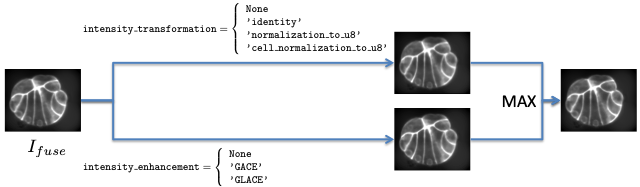
\includegraphics[height=50mm]{figures/build-input-segmentation.png}
\end{center}
\caption{\label{fig:cli:input:segmentation}
The input for segmentation (ie $h$-minima computation, seeded watershed) is built from (eventually) two images derived from the fusion image.}
\end{figure}


The segmentation of membranes images is based on a seeded watershed. Seeds are computed from either one single regional minima image (segmentation of the first time point, see section \ref{sec:cli:mars}) or several ones (segmentation by propagation of the other time points, see section \ref{sec:cli:astec}).


The regional minima operation, as well as the watershed operation, are conducted on the pre-processed version of the fused image. More precisely, the fused image may undergo two kinds of pre-processing, one denoted \option{intensity\_transformation} (and transform the image values based on its histogram) and the other \option{intensity\_enhancement} (and transform the image based on a membrane dedicated process). The image used for segmentation is the fusion (by the maximum) of these two pre-processing results (see figure \ref{fig:cli:input:segmentation}).

If the fused image is transformed before being segmented, the transformed image is named \texttt{<EN>\_fuse\_t<timepoint>\_membrane.inr} and stored in the directory \texttt{SEG/SEG\_<EXP\_SEG>/RECONSTRUCTION/} if the value of the variable \option{keep\_reconstruction} is set to \texttt{True}.

Note that specifying 
\begin{verbatim}
intensity_transformation = 'identity'
intensity_enhancement = None
\end{verbatim}
in the parameter file comes to use the unprocessed fused image as input image for the segmentation.


\subsection{Histogram based image value transformation}

The option \option{intensity\_transformation} can be set to one out the three (segmentation of the first time point, see section \ref{sec:cli:mars}) or four (segmentation by propagation of the other time points, see section \ref{sec:cli:astec}) values.
\begin{itemize}
\itemsep -0.5ex
\item \texttt{None}: this pre-processing channel is not used, meaning that only the membrane dedicated process will produce the input for the segmentation.
\item \texttt{'identity'}: there is no transformation of the fused image.
\item \texttt{'normalization\_to\_u8'}: input images are usually encoded on 2 bytes. However, it is of some interest to have input images of similar intensity distribution, so the segmentation parameters (eg the $h$'s for the regional minima computation) do not have to be tuned independently for each image or sequence.

This choice casts the input image on a one-byte image (ie into the value range $[0, 255]$) 
by linearly mapping the fused image values from $[I_{min}, I_{max}]$ to $[0, 255]$. $I_{min}$ and $I_{max}$ correspond respectively to the 1\% and to the 99\% percentiles of the fused image cumulative histogram. This allows to perform a robust normalization into $[0, 255]$ without being affected by extremely low or high intensity values.
Values below $I_{min}$ are set to $0$ while values above $I_{max}$ are set to $255$.

The percentiles used for the casting can be tuned by the means of two variables
\begin{verbatim}
normalization_min_percentile = 0.01
normalization_max_percentile = 0.99
\end{verbatim}

\item \texttt{'cell\_normalization\_to\_u8'}: this choice can only be used for the segmentation propagation (see section \ref{sec:cli:astec}). It has been developed (and kept) for historical reasons but has not proven to be useful yet. 
 
The segmentation (the image of cell labels) at time point $t$, $S^{\star}_t$, is first deformed onto the image at time $t+1$ thanks to the transformation $\mathcal{T}_{t \leftarrow t+1}$ from the image $I^{t+1}_{fuse}$ at time $t+1$ towards to image $I^{t}_{fuse}$ at time $t$ (this transformation is computed with the fused images). The deformed segmentation can be denoted by $S^{\star}_t \circ \mathcal{T}_{t \leftarrow t+1}$. 
According that the co-registration of the image $I^{t+1}_{fuse}$ and $I^{t}_{fuse}$ is successful, this deformed segmentation is an estimated segmentation (without any cell division) of $I^{t+1}_{fuse}$. 

Instead of computing one histogram for the whole image as in the \texttt{'normalization\_to\_u8'}, and thus having one $I_{min}$ and one $I_{max}$ value for the whole image, histogram are here computed on a cell basis, and a couple $(I_{min}, I_{max})$ is computed for each label of $S^{\star}_t \circ \mathcal{T}_{t \leftarrow t+1}$, yielding images of values $I_{min}$ and $I_{max}$. Since this induces discontinuities at cell borders, these two images are smoothed (with a Gaussian filter of standard deviation \option{cell\_normalization\_sigma} before casting into $[0, 255]$.

For each cell, different histogram can be used for the computation of $I_{min}$ and $I_{max}$.
\begin{itemize}
\itemsep -0.5ex
\item \option{cell\_normalization\_max\_method} sets the cell area where to compute the histogram for the $I_{max}$ value, while
\item \option{cell\_normalization\_min\_method} sets the cell area where to compute the histogram for the $I_{min}$ value.
\end{itemize}

Cell areas can be defined as
\begin{itemize}
\itemsep -0.5ex
\item \option{cell}: all the values of $I^{t+1}_{fuse}$ below the aimed cell defined in $S^{\star}_t \circ \mathcal{T}_{t \leftarrow t+1}$ are used for the histogram computation, 
\item \option{cellborder}: only the values of $I^{t+1}_{fuse}$ at the aimed cell border defined in $S^{\star}_t \circ \mathcal{T}_{t \leftarrow t+1}$ are used for the histogram computation, and 
\item \option{cellinterior}: all the value of $I^{t+1}_{fuse}$ in the aimed cell interior (the border is excluded) defined in $S^{\star}_t \circ \mathcal{T}_{t \leftarrow t+1}$ are used for the histogram computation.
\end{itemize}

Default values are 
\begin{verbatim}
cell_normalization_max_method = 'cellborder'
cell_normalization_min_method = 'cellinterior'
\end{verbatim}
meaning that $I_{max}$'s are computed at the cells' borders while $I_{min}$'s are computed in the cells' interiors. 
\end{itemize}


\subsection{Membrane dedicated enhancement}

The option \option{intensity\_transformation} can be set to one out the two (segmentation of the first time point, see section \ref{sec:cli:mars}) or three (segmentation by propagation of the other time points, see section \ref{sec:cli:astec}) values.

\begin{itemize}
\itemsep -0.5ex
\item \texttt{None}: this pre-processing channel is not used, meaning that only the histogram based image value transformation will produce the input for the segmentation.
\item \texttt{'GACE'} stands for \textit{Global Automated Cell Extractor}. This is the method described in \cite{michelin:hal-00915000,michelin:tel-01451608}.
\item \texttt{'GLACE'} stands for \textit{Grouped Local Automated Cell Extractor}. It differs from one step from \texttt{GACE}: the threshold of extrema image is not computed globally (as in \texttt{GACE}), but one threshold is computed per cell of $S^{\star}_t \circ \mathcal{T}_{t \leftarrow t+1}$, from the extrema values of the cell bounding box.
\end{itemize}

\texttt{GACE} and \texttt{GLACE} consist both of the following steps.

\begin{enumerate}
\itemsep -0.5ex

\item Membrane dedicated response computation. The Hessian is computed by convolution with the second derivatives of a Gaussian kernel (whose standard  deviation is given by \option{mars\_sigma\_membrane}). The analysis of eigenvalues and vectors of the Hessian matrix allows to recognize the normal direction of an eventual membrane. A response is then computed based on a contour detector in the membrane normal direction.

\item Directional extrema extraction. Extrema of the response in the direction of the membrane normal are extracted. It yields a valued image of membrane centerplanes.

\item \label{it:gace:threshold} Direction dependent automated thresholding.

It has been observed that the membrane contrast depends on the membrane orientation with respect to the microscope apparatus. Directional response histogram are built and a threshold is computed for each of them, which allows to compute a direction-dependent threshold. 

Thresholds are computing by fitting known distribution on histograms. Fitting is done by the means of an iterative minimization, after an automated initialization. The \option{mars\_sensitivity} option allows to control the threshold choice after the distribution fitting.

Setting the \option{mars\_manual} to \texttt{True} allows to manually initialize the distribution before minimization thanks to the \option{mars\_manual\_sigma} option.

Last, the user can directly give the threshold to be applied (this is then a global threshold that did not depend on the membrane direction) by setting the \option{mars\_hard\_thresholding} option at \texttt{True}: the threshold to be applied has to set at the \option{mars\_hard\_threshold} option.

\item Sampling. Points issued from the previous binarization step will be further used for a tensor voting procedure. To decrease the computational cost, only a fraction of the binary membrane may be retained. 
This fractions is set by the \option{mars\_sample} option.

Sampling is performed through pseudo-random numbers. To reproduce a  segmentation experiment by \texttt{2-mars.py}, the random seed can be set thanks to the \option{mars\_sample\_random\_seed} option.

If one want to reproduce segmentation experiments, 
the verboseness of the experiments has to be increased by adding at least one \option{-v} in the command line of \texttt{2-mars.py}. This ensures that the necessary information will be written into the \texttt{.log} file.
Then, to reproduce one given experiment, one has to retrieve the used random seed \texttt{'RRRRRRRRRR'} from the line 
\begin{verbatim}
Sampling step : random seed = RRRRRRRRRR
\end{verbatim}
in the log file 
\texttt{SEG/SEG\_<EXP\_SEG>/LOGS/2-mars-XXXX-XX-XX-XX-XX-XX.log}, and then to add the line
\begin{verbatim}
mars_sample_random_seed = 'RRRRRRRRRR'
\end{verbatim}
in the parameter file to get the same sampling.


\item \label{it:gace:tensorvoting} Tensor voting.
Each retained point of the binary image (together with its membrane normal direction) generates a tensor voting field, whose extent is controlled by the \option{mars\_sigma\_TV} option (expressed in voxel units). These fields are added to yield a global tensor image, and a membraness value is computed at each point, resulting in a scalar image.

\item Smoothing. An eventual last smoothing of this scalar image may be done, controlled by the \option{mars\_sigma\_LF} option.
\end{enumerate}





\subsection{Parameter list}

General parameters governing the segmentation pre-processing:
\begin{itemize}
\itemsep -0.5ex
%\item \texttt{EN}
\item \texttt{astec\_intensity\_enhancement}: equivalent to
      \texttt{intensity\_enhancement}
\item \texttt{astec\_intensity\_transformation}: equivalent to
      \texttt{intensity\_transformation}
\item \texttt{astec\_keep\_reconstruction}: equivalent to
      \texttt{keep\_reconstruction}
\item \texttt{intensity\_enhancement}
\item \texttt{intensity\_transformation}
\item \texttt{keep\_reconstruction}
\item \texttt{mars\_intensity\_enhancement}: equivalent to
      \texttt{intensity\_enhancement}
\item \texttt{mars\_intensity\_transformation}: equivalent to
      \texttt{intensity\_transformation}
\item \texttt{mars\_keep\_reconstruction}: equivalent to
      \texttt{keep\_reconstruction}
\end{itemize}

Parameters for the histogram based image value transformation:
\begin{itemize}
\itemsep -0.5ex
%\item \texttt{EN}
\item \texttt{astec\_cell\_normalization\_max\_method}: equivalent to
      \texttt{cell\_normalization\_max\_method}
\item \texttt{astec\_cell\_normalization\_min\_method}: equivalent to
      \texttt{cell\_normalization\_min\_method}
\item \texttt{astec\_cell\_normalization\_sigma}: equivalent to
      \texttt{cell\_normalization\_sigma}
\item \texttt{astec\_normalization\_max\_percentile}: equivalent to
      \texttt{normalization\_max\_percentile}
\item \texttt{astec\_normalization\_min\_percentile}: equivalent to
      \texttt{normalization\_min\_percentile}
\item \texttt{cell\_normalization\_max\_method}
\item \texttt{cell\_normalization\_min\_method}
\item \texttt{cell\_normalization\_sigma}
\item \texttt{mars\_normalization\_max\_percentile}: equivalent to
      \texttt{normalization\_max\_percentile}
\item \texttt{mars\_normalization\_min\_percentile}: equivalent to
      \texttt{normalization\_min\_percentile}
\item \texttt{normalization\_max\_percentile}
\item \texttt{normalization\_min\_percentile}
\end{itemize}

Parameters for the membrane dedicated enhancement;
\begin{itemize}
\itemsep -0.5ex
\item \texttt{astec\_hard\_threshold}: equivalent to
      \texttt{mars\_hard\_threshold}
\item \texttt{astec\_hard\_thresholding}: equivalent to
      \texttt{mars\_hard\_thresholding}
\item \texttt{astec\_manual}: equivalent to
      \texttt{mars\_manual}
\item \texttt{astec\_manual\_sigma}: equivalent to
      \texttt{mars\_manual\_sigma}
\item \texttt{astec\_sample}: equivalent to
      \texttt{mars\_sample}
\item \texttt{astec\_sample\_random\_seed}: equivalent to
      \texttt{mars\_sample\_random\_seed}
\item \texttt{astec\_sensitivity}: equivalent to
      \texttt{mars\_sensitivity}
\item \texttt{astec\_sigma\_LF}: equivalent to
      \texttt{mars\_sigma\_LF}
\item \texttt{astec\_sigma\_TV}: equivalent to
      \texttt{mars\_sigma\_TV}
\item \texttt{astec\_sigma\_membrane}: equivalent to
      \texttt{mars\_sigma\_membrane}
\item \texttt{mars\_hard\_threshold}
\item \texttt{mars\_hard\_thresholding}
\item \texttt{mars\_manual}
\item \texttt{mars\_manual\_sigma}
\item \texttt{mars\_sample}: this parameter sets the fraction of the binary centerplanes that will be used for tensor voting (step \ref{it:gace:tensorvoting}). Points being randomly drawn, results are not strictly reproducible if the code is re-run with the same sets of parameters. Using a larger value (smaller than or equal to 1.0) increases the reproductibility but induces a larger computational cost.
\item \texttt{mars\_sample\_random\_seed}: allows to set the random seed for reproductibility of the sampling step
\item \texttt{mars\_sensitivity}: this parameter sets the sensitivity for the centerplanes thresholding of step \ref{it:gace:threshold}. It is set to 0.99 by default. Using larger value (smaller than or equal to 1.0, say 0.9999) allows to extract less-contrasted membranes (for instance cell/background membranes).
\item \texttt{mars\_sigma\_LF}: expressed in real units
\item \texttt{mars\_sigma\_TV}: expressed in voxel units
\item \texttt{mars\_sigma\_membrane}: expressed in real units
\end{itemize}



%%%%%%%%%%%%%%%%%%%%%%%%%%%%%%%%%%%%%%%%%%%%%%%%%%%%%%%%%%%%
%
% parameters
%
%%%%%%%%%%%%%%%%%%%%%%%%%%%%%%%%%%%%%%%%%%%%%%%%%%%%%%%%%%%%

\section{Parameters}
\label{sec:cli:parameters}

\subsection{Data organisation parameters}

\subsection{Registration parameters}
\label{sec:cli:parameters:registration}

\begin{itemize}
\itemsep -0.5ex
\item \texttt{compute\_registration}
\item \texttt{pyramid\_highest\_level}
\item \texttt{pyramid\_lowest\_level}
\item \texttt{gaussian\_pyramid}
\item \texttt{transformation\_type}
\item \texttt{elastic\_sigma}
\item \texttt{transformation\_estimation\_type}
\item \texttt{lts\_fraction}
\item \texttt{fluid\_sigma}
\item \texttt{normalization}
\end{itemize}

